%%%% ijcai20.tex

\typeout{IJCAI--PRICAI--20 Instructions for Authors}

% These are the instructions for authors for IJCAI-20.

\documentclass{article}

\pdfpagewidth=8.5in
\pdfpageheight=11in
% The file ijcai20.sty is NOT the same than previous years'
\usepackage{ijcai20}

% Use the postscript times font!
\usepackage{times}
\usepackage{soul}
\usepackage{url}
\usepackage[hidelinks]{hyperref}
\usepackage[utf8]{inputenc}
\usepackage[small]{caption}
\usepackage{graphicx}
\usepackage{amsmath}
\usepackage{amsthm}
\usepackage{booktabs}
\usepackage{algorithm}
\usepackage{algorithmic}

\usepackage{CJKutf8}
\usepackage{diagbox}
\usepackage{multirow}
\usepackage{amsthm}
\usepackage{mathtools}
\usepackage{hhline}
\usepackage{booktabs}
\usepackage{tablefootnote}

\urlstyle{same}

% the following package is optional:
%\usepackage{latexsym} 

% See https://www.overleaf.com/learn/latex/theorems_and_proofs
% for a nice explanation of how to define new theorems, but keep
% in mind that the amsthm package is already included in this
% template and that you must *not* alter the styling.
\newtheorem{example}{Example}
\newtheorem{theorem}{Theorem}

% Following comment is from ijcai97-submit.tex:
% The preparation of these files was supported by Schlumberger Palo Alto
% Research, AT\&T Bell Laboratories, and Morgan Kaufmann Publishers.
% Shirley Jowell, of Morgan Kaufmann Publishers, and Peter F.
% Patel-Schneider, of AT\&T Bell Laboratories collaborated on their
% preparation.

% These instructions can be modified and used in other conferences as long
% as credit to the authors and supporting agencies is retained, this notice
% is not changed, and further modification or reuse is not restricted.
% Neither Shirley Jowell nor Peter F. Patel-Schneider can be listed as
% contacts for providing assistance without their prior permission.

% To use for other conferences, change references to files and the
% conference appropriate and use other authors, contacts, publishers, and
% organizations.
% Also change the deadline and address for returning papers and the length and
% page charge instructions.
% Put where the files are available in the appropriate places.

\title{CoCon: A Dataset of Short Chinese Phrases for Commonsense Contradiction Identification}

\iffalse
% Single author syntax
\author{
	Christian Bessiere
	\affiliations
	CNRS, University of Montpellier, France
	\emails
	pcchair@ijcai20.org
}
\fi

% Multiple author syntax (remove the single-author syntax above and the \iffalse ... \fi here)
% Check the ijcai20-multiauthor.tex file for detailed instructions
\iffalse
\author{
	First Author$^1$
	\and
	Second Author$^2$\and
	Third Author$^{2,3}$\And
	Fourth Author$^4$
	\affiliations
	$^1$First Affiliation\\
	$^2$Second Affiliation\\
	$^3$Third Affiliation\\
	$^4$Fourth Affiliation
	\emails
	\{first, second\}@example.com,
	third@other.example.com,
	fourth@example.com
}
\fi

\newcommand{\JQ}[1]{\textcolor{blue}{JQ: #1}}
\newcommand{\KZ}[1]{\textcolor{red}{Kenny: #1}}



\begin{document}
	\maketitle
	\begin{abstract}
		Incorporating commonsense knowledge to machines is a long-standing challenge to fulfill real artificial intelligence. Given that mobile users tend to generate shorter content, we target common sense on short, context-poor phrases, unlike previous researches which mainly focus on commonsense inferences between long contents. With the help of our constructed \textit{Concept Association Graph} which contains abundant web knowledge, we propose a new dataset \textbf{CoCon} with over 9,000 pairs of short Chinese phrases, which is designed for testing the capability of machines on commonsense reasoning. Preliminary experiments show that large pre-trained language models such as BERT and ERNIE are still lagging behind human performance by a large margin on CoCon, which indicates that further efforts are needed to enable machines to grasp such commonsense knowledge. 
	\end{abstract}

	\begin{CJK}{UTF8}{gbsn}
	%\IEEEraisesectionheading{
% %\IEEEraisesectionheading{
% %\IEEEraisesectionheading{
% \input{intro}
\section{Introduction}\label{sec:intro}
 %}
% \section{Introduction}\label{sec:intro}

% \begin{enumerate}
% \item Motivation: application scenarios (with 1-2 running examples);
% \item Characteristics of the data sources and their challenges;
% \item Briefly introduce previous approaches to extract information 
% from images including setting the document zone, and their limitations.
% \item General flow of our approach (may give a diagram here)
% \end{enumerate}
% scenary

Due to ever evolving hardware and software, many medical images
such as electro-cardio graphs (ECGs), X-ray or ultrasound images  
are directly printed and stored in hard copy formats. 
% \KZ{Insert 4 example images here.}
%Examples are shown in \figref{fig:medicalImages}. 
% These images often contain a mix of graphics and text, which
% include parameter settings of the hardware, test measurements or simple
% diagnosis. 
These images often contain a mix of graphics and text, which 
include technical settings of the hardware used, test measurements or simple diagnoses.
Recently, there has been a growing demand for digitizing such 
medical information from paper media sources, especially legacy ones, or patients who want to keep track of these documents by themselves digitally. 
Apart from scanning the graphics into a digital format, extracting 
the semi-structured textual information is also an important part of
building electronic medical records for patients. 

%\begin{figure}[!htb]
%\centering
%\subfloat[ECG]{
%\label{fig:medicalimage:ecg}
%\epsfig{file=figure/17_ori.eps, width=0.4\columnwidth}
%}
%% \hfill
%\subfloat[MRI]{
%	\label{fig:medicalimage:mrt}
%	\epsfig{file=figure/MRI.eps, width=0.4\columnwidth}
%}
%\\
%\subfloat[X-RAY]{
%\label{fig:medicalimage:xray}
%\epsfig{file=figure/X-RAY.eps, width=0.4\columnwidth}
%}
%%\hfill
%\subfloat[EEG]{
%\label{fig:medicalimage:eeg}
%\epsfig{file=figure/EEG.eps, width=0.4\columnwidth}
%}
%\caption{Examples of Medical Images}
%\label{fig:medicalImages}
%\end{figure}

Optical character recognition (OCR)  \cite{mori1992historical,smith2007overview} is 
a traditional technique used to turn images of printed text into machine encoded
text. It is well researched and performs well on plain text 
documents such as novels and reports, for a variety of languages. 
%For example, Tesseract, which is one of 
%the most popular open source multilingual recognizers, logs an error 
%rate of 3.72\% for English words and 3.77\% for simplified 
%Chinese characters\cite{smith2009adapting}. 
%Google Books \cite{googlebooks} and Gutenberg \cite{gutenberg} are
%projects which have scanned a large number of paper books into text for free and open
%access. These projects made exclusive use of OCR for this conversion and 
%achieved high accuracy \cite{vincent2007google} \cite{lebert2008project}. 
% 99\% for Gutenberg project \cite{lebert2008project}. 
% \KZ{Give the accuracy of google and gutenberg if available.}


\begin{figure}[th]
\centering
\epsfig{file=figure/17_b.eps, width=0.8\columnwidth}
\caption{An ECG image with text area (red circle) of interest.}
\label{fig:ecgexample2}
\end{figure}

For a semi-structured medical image, such as 
\figref{fig:ecgexample2}, we would like to extract the attribute-value 
pairs (e.g., {\em Vent. rate = 63 bpm}) and possibly other values such as
date ({\em 18-Nov-2010}) and time ({\em 9:13:02}) since those values endow us with lots of information about the patient. 
Existing OCR software cannot extract such structured information in a straightforward 
fashion, 
but instead it produces rather convoluted results from the whole image, 
similar to those in \figref{fig:ocrre}, which was produced by Tesseract, 
a popular multi-lingual recognizers. 
% \KZ{Maybe include the x-y coordinate info in the output as well?}  

\begin{figure}[th]
\centering
\scriptsize
\begin{verbatim}
<p class="ocr_par" title="box 263 33 444 119">
   <span class="ocr_l" title="box 264 33 336 45">
       <span class="ocrx_w" title="box 264 33 299 45">Vcnt.</span> 
       <span class="ocrx_w" title="box 308 34 336 45">rule</span> 
   </span>
   <span class='ocr_l'>
       <span class="ocrx_w" title="box 264 51 283 64">PR</span> 
       <span class="ocrx_w" title="box 291 51 346 64">Interval</span> 
       <span class="ocrx_w" title="box 389 52 411 64">140</span> 
       <span class="ocrx_w" title="box 420 55 439 64">ms</span> 
   </span>
   ...
   </span>
</p>
<p class="ocr_p" dir="ltr">
   <span class="ocr_l">
       <span class="ocrx_w" title="box 396 33 411 45">53</span> 
       <span class="ocrx_w" title="box 420 33 449 48">bpm</span> 
   </span>
</p>
\end{verbatim}
\caption{Snippet OCR results in XML, input to our framework.}
\label{fig:ocrre}
\end{figure}


%\input{xmlre1}

%However, OCR alone does not work well on semi-structured text and hence
%can't be directly used for information extraction from the aforementioned
%medical images. \KZ{Give the reason here, perhaps because OCR models are
%largely Markov based? So semi-structured data breaks the flow of text.}
%When a medical image is input to an ordinary OCR software, the spatial 
%information of the text components is often lost or mixed with noises
%and errors.
%%The reason is OCR converts the whole images into text data, in which 
%%useful information often mix with noises and errors. 
%In this paper, we would like to extract the attribute-value pairs
%and possibly other values from \figref{fig:ecgexample1} 
%and \figref{fig:ecgexample2}. 
%% or medical ultrasonography report. 
%Such images contain lots of non-textual information or noises.

% example & ref
%\begin{figure}[ht]
%\centering
%\epsfig{file=figure/46.eps, width=0.8\columnwidth}
%\caption{ECG Images From Printer1}
%\label{fig:ecgexample1}
%\end{figure}

% \begin{figure}[ht]
% \centering
% \subfloat[Printer1]{
% \label{fig:ecgexample:a}
% \epsfig{file=figure/46.eps, width=0.48\columnwidth}
% }
% \hfill
% \subfloat[Printer2]{
% \label{fig:ecgexample:b}
% \epsfig{file=figure/17.eps, width=0.48\columnwidth}
% }
% \caption{ECG images from two different printers}
% \label{fig:ecgexample}
% \end{figure}

Also, errors in the OCR text \cite{darwish2007error,taghva1996evaluation} will greatly affect the effectiveness 
of other related tasks. Much work has been done to improve the performance of the OCR\cite{kolak2003generative,cesarini1998informys}. However, there are still a number of significant challenges involved in extracting the information from medical images or OCR results in XML form. 

% First, medical images differ from pure text document in that them have 
% layout information. 
First, medical images differ from pure text documents in that 
they contain layout information.
Although most current OCR engines attempt to reproduce the physical 
layout of the text units, 
%(along with X-Y coordinates) and store them 
%in a special format such as XML 
% (\KZ{Better in the previous example})
such spatial
information is approximate and sometimes inaccurate, which is why neighboring
text blocks in \figref{fig:ecgexample2}, such as ``Vent. Rate'' and
``63 bpm'' were not automatically combined into the same XML block, but were 
rather far apart (shown in two different ``classes'') in \figref{fig:ocrre} made by OCR softwares. 
%Even for images produced by the same ECG printer, 
%the XML results can still be very different as 
The spatial layout is sensitive to many factors, such as accidental spots 
on the prints, color and contrast, or the angle of the camera. 
%In this case, solutions for other application domains, for example, the web, 
%are not well suited for information extraction from printed documents \cite{bartoli2014semisupervised}. With such inaccurate
%layout information produced by OCR,
%it is not easy to write a simple wrapper program to extract useful
%data from images, even if the images come from the same printer. 

%Writing a wrapper for each
%individual image would be tedious and counter-productive. Therefore,
%a mechanism that makes use of the spatial locality of the 
%text units in the image and 
%accommodates slight variations in the spatial layout would make the extraction
%more accurate and fault-tolerant.

%For example, \figref{fig:ocrre} is the simplified OCR results for the ECGs in 
%\figref{fig:ecgexample1} and \figref{fig:ecgexample2}. The results are in the XML format and have attritube named {\em class} 
%for layout information. Although these two images share similar format. 
%OCR engine generates different results in that it splits elements that 
%should be in the same line into two lines in the second example. 
%XML is sensitive to the layout results so it's hard to tolerate 
%all the layout results. 
%
% example check the term
% layout of ocr results can be restore, so why OCR engine don't restore the results 
% using the similar methods as we do?
% or the way we handle the layout problem is quite simple

% Delete for TIP
% Second, exiting OCR engines make heavy use of Markov properties such as n-grams
% since they primarily target the transformation of large body of text 
% \cite{kolak2003generative}. 
% % \KZ{Needs some refs here.}
% Unfortunately, the semi-structured texts in medical images are often 
% short and not even written in complete sentences, thus breaking Markov assumption. To make
% matters worse, medical images contain scientific language, which may be
% very different from the training corpora of these OCR engines.
% This explains why we see errors like ``Vcnt'' and ``rule'' 
% in \figref{fig:ocrre}. 
% %can't guarantee a perfect performance, which means 
% %there are errors and noises in the OCR results.
% %Many of them due to the fact that the data are no longer long, continous
% %sentences, thus breaking the Markov assumption made by many OCR algorithms. 
% %In \figref{fig:ocrresub:b}, ``Vent." is misrecognized as ``Vcnt.". 
% Without sufficient contextual information, OCR may also misrecognize a 
% digit as an alphabetic character, or as another similar digit. 
% Furthermore, the mix of text with images and formatting
% lines often confuses the OCR engine, which is more biased toward full
% text images.
% Exact pattern matching, as used in
% traditional information extraction, doesn't work with such noisy OCR output
% as it doesn't tolerate noises or errors in text. 
% %It's hard to autocorrect these errors 
% %because image quality is the most important affecting factor. 
% %The text we are processing can be full of no meaning words or 
% %strange numbers. 
% A fuzzy matching strategy is more desirable in this case. 
% % example, what are the traditional IEs

Second, there are many types of medical images, resulting from a variety of
medical tests. Different equipments for the same test can produce vastly 
different images. Writing individual extraction wrappers 
for the OCR outputs of all these formats is tedious and inefficient, 
and difficult for non-programmers.
%not to mention that there are significant programming barriers for 
%writing these wrappers, especially for the medical professionals who are the
%end users of these extraction results. 
%A more user-friendly approach enabling users to specify such extraction requirements would be preferred. 
%There are various kinds of medical images, such as electrocardiograph report, 
%medical ultrasonography report, etc. 
%However the basic measures for each type of medical test (e.g., ECG), 
%are very similar from machine to machine. Only the layouts are 
%different. 
% example medical images

Finally, most off-the-shelf OCR programs are pre-trained with specific 
recognition models, which may not be suitable for the extraction of 
%medical images.
%Furthermore, changes in imaging equipment technology over time may produce 
%different formats, layout, or terminology, rendering existing OCR models 
%obsolete. 
Re-training the models requires a large amount of labeled data, which may
not be available. 
%Incremental training as more labeled data arrives
%is currently not supported by any OCR product.    

%There have been some limited attempts to address some of the above challenges. 
%One solution is a plugin of an OCR program that allows the user to specify 
%target zones of interest in the image to be extracted. The zones specified for
%one image can be applied to images with slight variations by adjusting against
%a fixed reference point that is supposed to exist in all these images.
%% \KZ{I think the problem is not so much with the zones, because we also
%% have zones, but rather with the reference point.}
%% \JY{}
%% example products
%% http://www.square-9.com/automated-data-extraction-optical-character-recognition
%The problem with this solution is its high reliance on the OCR zones  
%established by the user. The performance of the results is affected by the 
%accuracy of the zones. If the zones are too big, the results will be full of 
%noise. If the zones are too small, results will miss something. 
%
%Another solution involves using the page layout analysis technique. The page layout 
%analysis technique is used to determine where the text 
%resides on a page \cite{o1993document}, 
%% \KZ{This page layout analysis approach is not clearly described. I don't understand after reading this paragraph.}
%% By using page layout analysis technique, the hierarchy of physical components 
%% can be generated and to match with the hierarchy of logical components, which 
%% is predefined. 
%this includes identifying and categorizing the 
%regions of interest in the scanned image of a text document. 
%Typically, the first step is to segment text zones from 
%non-textual zones and arrange them in their original order. 
%Then in order to analyze the logical roles of the text zones 
%(titles, captions, footnotes, etc.), logical layout analysis 
%is used for labeling the semantics of the text zones.
%Generally, page layout analysis is used for documents. The problem with applying 
%such a technique on medical images is that it creates so much noises 
%that performance is ultimately affected. 
%For medical imaging reports like ECG, useful information is often 
%found in the small components of the image, while most of the images are 
%read as noises. 
% check paper and more description, weakness, ref

%In this paper, 
%we propose a spatial data description language, which borrows its syntax from
%PADS \cite{fisher+:pads}, an ad hoc data processing language, 
%for describing semi-structured data in medical images. 
%% ref
%We call this language OCR description language, or ODL. 
%ODL is designed for extracting and parsing semi-structured text data 
%from images. We believe that  information extraction from those data in ODL form may be much easier than extracting information from rough data or data in XML form, which means that our preprocessing part proves to be necessary.
%%An example ODL description for the image in 
%%\figref{fig:ecgexample2} is shown in 
%%\figref{fig:description}. \KZ{Make this description two column, and give
%%some brief explanation of this description here.} 
%%The parsing result of this description is shown
%%in \figref{fig:parsing result}. \KZ{Give some explanation of the results,
%%otherwise don't show the result here. E.g., you need to explain what F, E, etc.
%%mean. You want to say that even though rate has been recognized as rule,
%%the bpm value was still extracted (but still wrong!).}
%% \KZ{I removed the preprocessing part, cos it's not important. Talk about it in
%% discussion sec.}
%%The our approach starts by preprocessing the images for text results.
%To use this framework, the user first describes the components in the image
%that he or she is interested in extracting. This includes constant strings
%and variables of different data types.   
%ODL allows the user to specify the approximate spatial layout and constraints on
%the data, e.g., integers within 
%a certain range, real numbers with certain decimal points, etc. 
%%This information is then as the key component in our fuzzy matching strategy. 
%The system then automatically generates a parser for these medical images.
%This parser uses the output XML from OCR with spatial information as an input, 
%and outputs a data structure with values extracted for each variables
%in the description, unless there is an unrecoverable error during the parsing process.
%In addition, approximate layout information and constraints are used in parsing process 
%to tolerate noises and small format variations in the input images. 
%%Specifically, this method could be called fuzzy matching, meaning that more candidates could be saved after the parsing process.  It's obvious that we may have a higher probability to obtain the accurate result if more candidates are kept so that fuzzy match should be used properly in our system.
%%An autogenerated parser based on the ODL description can release us from 
%%repetitive work. In this way, we turn the task of writing complex parsers 
%%into describing information on images.
%
%
%When users process many images of the same format, the system 
%automatically discovers parsing errors given the current model and 
%prompts the user to manually correct some of the frequent and prominent
%errors, which effectively serves as an online labeling function. 
%These incrementally labeled data are then used to update the parsing model. 


%It should be emphasized that the incremental learning model is very important in our whole system. Incremental learning is a machine learning paradigm where the learning process takes place whenever we have new examples or data added to our baisc data set, leading to a most striking difference between incremental learning and traditional machine learning: it does not assume the availability of a sufficient training set before the learning process. What incremental learning in our system is really impressive: it does not require a relatively good and stable training set at first time. In fact, it could improve the parsing result with even relatively rough training sets at first by absorbing new data or corrective information as time passes in dynamic systems. Besides, the process would be very effective when there are some new images coming in since training process would not learn from scratch, which might waste time and computation resource.

%At last, we propose an incrementally human correction framwork which can 
%make the best use of human correction to handle the misrecognition problem. 
% Base on our experiments on about 500 real life ECG images, 
% our approach achieves p1 and p2 after p3 times human correction. 
% experimental results

% \begin{figure}[h]
% \begin{lstlisting}
% Oenum str_month_t{
% 	"Jan", "Feb", "Mar", "Apr",
% 	"May", "Jun", "Jul", "Aug",
% 	"Sept", "Oct", "Nov", "Dec"
% };

% Ounion month_t{
% 	Oint(1,12)	num;
% 	str_month_t	str;
% };

% Ostruct time_t{
% 	Oint(1,31)	day;
% 	"-";
% 	month_t	month;
% 	"-";
% 	Oint	year;
% };

% Ostruct triple_t{
% 	"Vent.";
% 	hskip(\s)	skip1;
% 	"rate";
% 	Oint x;
% 	"bpm";
% 	vskip(\n)	skip2;
% };

% Oscource Ostruct entry_t{
% 	time_t(<-,-,-,0.3l>) t;
% 	triple_t(<0.1w,-,0.5w,->) d;
% };
% \end{lstlisting}
% \caption{Description}\label{fig:description}
% \end{figure}


In order to solve above problems, We design a system which makes three main contributions:
\begin{enumerate}
\item Based on some previous work on data description language \cite{lamport1986document,taft1999post,fisher+:pads},we design a new declarative spatial data description language called \textit{OCR description language}, or ODL,
which allows users to specify spatial and data constraints in medical 
images(\secref{sec:syntax});
\item We propose a noise-tolerant parser which takes OCR results
the ODL description as input and outputs a data structure with values 
extracted for each variables in the description (\secref{sec:semantics});
\item We propose an incremental manual correction 
framework\cite{von2008recaptcha,zhu2012learnpads++}, which 
takes advantage of user corrections  and improves the productivity
significantly (\secref{sec:correction}).
%To be more specific, the framework improves the traditional machine learning methods by using a incremental learning process to avoid starting from scratch when we are trying to apply human corrections in the system. That means the framework would be more effective than most corrective systems.
\end{enumerate}


\section{Introduction}\label{sec:intro}
 %}
% \section{Introduction}\label{sec:intro}

% \begin{enumerate}
% \item Motivation: application scenarios (with 1-2 running examples);
% \item Characteristics of the data sources and their challenges;
% \item Briefly introduce previous approaches to extract information 
% from images including setting the document zone, and their limitations.
% \item General flow of our approach (may give a diagram here)
% \end{enumerate}
% scenary

Due to ever evolving hardware and software, many medical images
such as electro-cardio graphs (ECGs), X-ray or ultrasound images  
are directly printed and stored in hard copy formats. 
% \KZ{Insert 4 example images here.}
%Examples are shown in \figref{fig:medicalImages}. 
% These images often contain a mix of graphics and text, which
% include parameter settings of the hardware, test measurements or simple
% diagnosis. 
These images often contain a mix of graphics and text, which 
include technical settings of the hardware used, test measurements or simple diagnoses.
Recently, there has been a growing demand for digitizing such 
medical information from paper media sources, especially legacy ones, or patients who want to keep track of these documents by themselves digitally. 
Apart from scanning the graphics into a digital format, extracting 
the semi-structured textual information is also an important part of
building electronic medical records for patients. 

%\begin{figure}[!htb]
%\centering
%\subfloat[ECG]{
%\label{fig:medicalimage:ecg}
%\epsfig{file=figure/17_ori.eps, width=0.4\columnwidth}
%}
%% \hfill
%\subfloat[MRI]{
%	\label{fig:medicalimage:mrt}
%	\epsfig{file=figure/MRI.eps, width=0.4\columnwidth}
%}
%\\
%\subfloat[X-RAY]{
%\label{fig:medicalimage:xray}
%\epsfig{file=figure/X-RAY.eps, width=0.4\columnwidth}
%}
%%\hfill
%\subfloat[EEG]{
%\label{fig:medicalimage:eeg}
%\epsfig{file=figure/EEG.eps, width=0.4\columnwidth}
%}
%\caption{Examples of Medical Images}
%\label{fig:medicalImages}
%\end{figure}

Optical character recognition (OCR)  \cite{mori1992historical,smith2007overview} is 
a traditional technique used to turn images of printed text into machine encoded
text. It is well researched and performs well on plain text 
documents such as novels and reports, for a variety of languages. 
%For example, Tesseract, which is one of 
%the most popular open source multilingual recognizers, logs an error 
%rate of 3.72\% for English words and 3.77\% for simplified 
%Chinese characters\cite{smith2009adapting}. 
%Google Books \cite{googlebooks} and Gutenberg \cite{gutenberg} are
%projects which have scanned a large number of paper books into text for free and open
%access. These projects made exclusive use of OCR for this conversion and 
%achieved high accuracy \cite{vincent2007google} \cite{lebert2008project}. 
% 99\% for Gutenberg project \cite{lebert2008project}. 
% \KZ{Give the accuracy of google and gutenberg if available.}


\begin{figure}[th]
\centering
\epsfig{file=figure/17_b.eps, width=0.8\columnwidth}
\caption{An ECG image with text area (red circle) of interest.}
\label{fig:ecgexample2}
\end{figure}

For a semi-structured medical image, such as 
\figref{fig:ecgexample2}, we would like to extract the attribute-value 
pairs (e.g., {\em Vent. rate = 63 bpm}) and possibly other values such as
date ({\em 18-Nov-2010}) and time ({\em 9:13:02}) since those values endow us with lots of information about the patient. 
Existing OCR software cannot extract such structured information in a straightforward 
fashion, 
but instead it produces rather convoluted results from the whole image, 
similar to those in \figref{fig:ocrre}, which was produced by Tesseract, 
a popular multi-lingual recognizers. 
% \KZ{Maybe include the x-y coordinate info in the output as well?}  

\begin{figure}[th]
\centering
\scriptsize
\begin{verbatim}
<p class="ocr_par" title="box 263 33 444 119">
   <span class="ocr_l" title="box 264 33 336 45">
       <span class="ocrx_w" title="box 264 33 299 45">Vcnt.</span> 
       <span class="ocrx_w" title="box 308 34 336 45">rule</span> 
   </span>
   <span class='ocr_l'>
       <span class="ocrx_w" title="box 264 51 283 64">PR</span> 
       <span class="ocrx_w" title="box 291 51 346 64">Interval</span> 
       <span class="ocrx_w" title="box 389 52 411 64">140</span> 
       <span class="ocrx_w" title="box 420 55 439 64">ms</span> 
   </span>
   ...
   </span>
</p>
<p class="ocr_p" dir="ltr">
   <span class="ocr_l">
       <span class="ocrx_w" title="box 396 33 411 45">53</span> 
       <span class="ocrx_w" title="box 420 33 449 48">bpm</span> 
   </span>
</p>
\end{verbatim}
\caption{Snippet OCR results in XML, input to our framework.}
\label{fig:ocrre}
\end{figure}


%% \begin{figure}[ht]
% \centering
% \subfigure[]{
% \label{fig:subfig:a}
% \begin{minipage}[b]{0.2\textwidth}
%\newsavebox{\firstlisting}
%\begin{lrbox}{\firstlisting}% Store first listing
%\begin{lstlisting}
%<p class='ocr_par' dir='ltr'>
%   <span class='ocr_line' id='line_2'>
%       <span class='ocrx_word' id='word_6'>Vent.</span>
%       <span class='ocrx_word' id='word_7'>rate</span>
%       <span class='ocrx_word' id='word_8'>65</span>
%       <span class='ocrx_word' id='word_9'>bpm</span>
%   </span>
%   <span class='ocr_line' id='line_3'>
%       <span class='ocrx_word' id='word_14'>PR</span>
%       <span class='ocrx_word' id='word_15'>interval</span>
%       <span class='ocrx_word' id='word_16'>162</span>
%       <span class='ocrx_word' id='word_17'>ms</span>
%   </span>
%    ...
%</p>
%\end{lstlisting}
%\end{lrbox}
% \end{minipage}
% }
% \hspace[1in]
% \subfigure[]{
% % \label{fig:subfig:b}
% % \begin{minipage}[b]{0.2\textwidth}
\newsavebox{\secondlisting}
\begin{lrbox}{\secondlisting}
% \tiny
\begin{lstlisting}[basicstyle=\tiny,]
<p class="ocr_par" title="box 263 33 444 119">
   <span class="ocr_l" title="box 264 33 336 45">
       <span class="ocrx_w" title="box 264 33 299 45">Vcnt.</span>
       <span class="ocrx_w" title="box 308 34 336 45">rule</span>
   </span>
   <span class='ocr_l'>
       <span class="ocrx_w" title="box 264 51 283 64">PR</span>
       <span class="ocrx_w" title="box 291 51 346 64">Interval</span>
       <span class="ocrx_w" title="box 389 52 411 64">140</span>
       <span class="ocrx_w" title="box 420 55 439 64">ms</span>
   </span>
   ...
   </span>
</p>
<p class="ocr_p" dir="ltr">
   <span class="ocr_l">
       <span class="ocrx_w" title="box 396 33 411 45">53</span>
       <span class="ocrx_w" title="box 420 33 449 48">bpm</span>
   </span>
</p>
\end{lstlisting}
\end{lrbox}
% % \end{minipage}
% }

% \KZ{\figref{fig:ocrre} is output from what software? Tesseract?}
\begin{figure*}[th]
%\subfloat[Image From Printer1]{
%\label{fig:ocrresub:a}
%\scalebox{0.8}{\usebox{\firstlisting}}}
%\hfill
%\subfloat[Image From Printer2]{
\scalebox{1.6}{\usebox{\secondlisting}}
% \label{fig:ocrre}
\caption{A fragment of raw OCR results for ECG with layout information.}
%\caption{Simplified OCR Results in XML for an ECG with Layout Information}
%\label{fig:ocrresub:b}
\label{fig:running-xml}
\end{figure*}

% \lipsum[2]


%However, OCR alone does not work well on semi-structured text and hence
%can't be directly used for information extraction from the aforementioned
%medical images. \KZ{Give the reason here, perhaps because OCR models are
%largely Markov based? So semi-structured data breaks the flow of text.}
%When a medical image is input to an ordinary OCR software, the spatial 
%information of the text components is often lost or mixed with noises
%and errors.
%%The reason is OCR converts the whole images into text data, in which 
%%useful information often mix with noises and errors. 
%In this paper, we would like to extract the attribute-value pairs
%and possibly other values from \figref{fig:ecgexample1} 
%and \figref{fig:ecgexample2}. 
%% or medical ultrasonography report. 
%Such images contain lots of non-textual information or noises.

% example & ref
%\begin{figure}[ht]
%\centering
%\epsfig{file=figure/46.eps, width=0.8\columnwidth}
%\caption{ECG Images From Printer1}
%\label{fig:ecgexample1}
%\end{figure}

% \begin{figure}[ht]
% \centering
% \subfloat[Printer1]{
% \label{fig:ecgexample:a}
% \epsfig{file=figure/46.eps, width=0.48\columnwidth}
% }
% \hfill
% \subfloat[Printer2]{
% \label{fig:ecgexample:b}
% \epsfig{file=figure/17.eps, width=0.48\columnwidth}
% }
% \caption{ECG images from two different printers}
% \label{fig:ecgexample}
% \end{figure}

Also, errors in the OCR text \cite{darwish2007error,taghva1996evaluation} will greatly affect the effectiveness 
of other related tasks. Much work has been done to improve the performance of the OCR\cite{kolak2003generative,cesarini1998informys}. However, there are still a number of significant challenges involved in extracting the information from medical images or OCR results in XML form. 

% First, medical images differ from pure text document in that them have 
% layout information. 
First, medical images differ from pure text documents in that 
they contain layout information.
Although most current OCR engines attempt to reproduce the physical 
layout of the text units, 
%(along with X-Y coordinates) and store them 
%in a special format such as XML 
% (\KZ{Better in the previous example})
such spatial
information is approximate and sometimes inaccurate, which is why neighboring
text blocks in \figref{fig:ecgexample2}, such as ``Vent. Rate'' and
``63 bpm'' were not automatically combined into the same XML block, but were 
rather far apart (shown in two different ``classes'') in \figref{fig:ocrre} made by OCR softwares. 
%Even for images produced by the same ECG printer, 
%the XML results can still be very different as 
The spatial layout is sensitive to many factors, such as accidental spots 
on the prints, color and contrast, or the angle of the camera. 
%In this case, solutions for other application domains, for example, the web, 
%are not well suited for information extraction from printed documents \cite{bartoli2014semisupervised}. With such inaccurate
%layout information produced by OCR,
%it is not easy to write a simple wrapper program to extract useful
%data from images, even if the images come from the same printer. 

%Writing a wrapper for each
%individual image would be tedious and counter-productive. Therefore,
%a mechanism that makes use of the spatial locality of the 
%text units in the image and 
%accommodates slight variations in the spatial layout would make the extraction
%more accurate and fault-tolerant.

%For example, \figref{fig:ocrre} is the simplified OCR results for the ECGs in 
%\figref{fig:ecgexample1} and \figref{fig:ecgexample2}. The results are in the XML format and have attritube named {\em class} 
%for layout information. Although these two images share similar format. 
%OCR engine generates different results in that it splits elements that 
%should be in the same line into two lines in the second example. 
%XML is sensitive to the layout results so it's hard to tolerate 
%all the layout results. 
%
% example check the term
% layout of ocr results can be restore, so why OCR engine don't restore the results 
% using the similar methods as we do?
% or the way we handle the layout problem is quite simple

% Delete for TIP
% Second, exiting OCR engines make heavy use of Markov properties such as n-grams
% since they primarily target the transformation of large body of text 
% \cite{kolak2003generative}. 
% % \KZ{Needs some refs here.}
% Unfortunately, the semi-structured texts in medical images are often 
% short and not even written in complete sentences, thus breaking Markov assumption. To make
% matters worse, medical images contain scientific language, which may be
% very different from the training corpora of these OCR engines.
% This explains why we see errors like ``Vcnt'' and ``rule'' 
% in \figref{fig:ocrre}. 
% %can't guarantee a perfect performance, which means 
% %there are errors and noises in the OCR results.
% %Many of them due to the fact that the data are no longer long, continous
% %sentences, thus breaking the Markov assumption made by many OCR algorithms. 
% %In \figref{fig:ocrresub:b}, ``Vent." is misrecognized as ``Vcnt.". 
% Without sufficient contextual information, OCR may also misrecognize a 
% digit as an alphabetic character, or as another similar digit. 
% Furthermore, the mix of text with images and formatting
% lines often confuses the OCR engine, which is more biased toward full
% text images.
% Exact pattern matching, as used in
% traditional information extraction, doesn't work with such noisy OCR output
% as it doesn't tolerate noises or errors in text. 
% %It's hard to autocorrect these errors 
% %because image quality is the most important affecting factor. 
% %The text we are processing can be full of no meaning words or 
% %strange numbers. 
% A fuzzy matching strategy is more desirable in this case. 
% % example, what are the traditional IEs

Second, there are many types of medical images, resulting from a variety of
medical tests. Different equipments for the same test can produce vastly 
different images. Writing individual extraction wrappers 
for the OCR outputs of all these formats is tedious and inefficient, 
and difficult for non-programmers.
%not to mention that there are significant programming barriers for 
%writing these wrappers, especially for the medical professionals who are the
%end users of these extraction results. 
%A more user-friendly approach enabling users to specify such extraction requirements would be preferred. 
%There are various kinds of medical images, such as electrocardiograph report, 
%medical ultrasonography report, etc. 
%However the basic measures for each type of medical test (e.g., ECG), 
%are very similar from machine to machine. Only the layouts are 
%different. 
% example medical images

Finally, most off-the-shelf OCR programs are pre-trained with specific 
recognition models, which may not be suitable for the extraction of 
%medical images.
%Furthermore, changes in imaging equipment technology over time may produce 
%different formats, layout, or terminology, rendering existing OCR models 
%obsolete. 
Re-training the models requires a large amount of labeled data, which may
not be available. 
%Incremental training as more labeled data arrives
%is currently not supported by any OCR product.    

%There have been some limited attempts to address some of the above challenges. 
%One solution is a plugin of an OCR program that allows the user to specify 
%target zones of interest in the image to be extracted. The zones specified for
%one image can be applied to images with slight variations by adjusting against
%a fixed reference point that is supposed to exist in all these images.
%% \KZ{I think the problem is not so much with the zones, because we also
%% have zones, but rather with the reference point.}
%% \JY{}
%% example products
%% http://www.square-9.com/automated-data-extraction-optical-character-recognition
%The problem with this solution is its high reliance on the OCR zones  
%established by the user. The performance of the results is affected by the 
%accuracy of the zones. If the zones are too big, the results will be full of 
%noise. If the zones are too small, results will miss something. 
%
%Another solution involves using the page layout analysis technique. The page layout 
%analysis technique is used to determine where the text 
%resides on a page \cite{o1993document}, 
%% \KZ{This page layout analysis approach is not clearly described. I don't understand after reading this paragraph.}
%% By using page layout analysis technique, the hierarchy of physical components 
%% can be generated and to match with the hierarchy of logical components, which 
%% is predefined. 
%this includes identifying and categorizing the 
%regions of interest in the scanned image of a text document. 
%Typically, the first step is to segment text zones from 
%non-textual zones and arrange them in their original order. 
%Then in order to analyze the logical roles of the text zones 
%(titles, captions, footnotes, etc.), logical layout analysis 
%is used for labeling the semantics of the text zones.
%Generally, page layout analysis is used for documents. The problem with applying 
%such a technique on medical images is that it creates so much noises 
%that performance is ultimately affected. 
%For medical imaging reports like ECG, useful information is often 
%found in the small components of the image, while most of the images are 
%read as noises. 
% check paper and more description, weakness, ref

%In this paper, 
%we propose a spatial data description language, which borrows its syntax from
%PADS \cite{fisher+:pads}, an ad hoc data processing language, 
%for describing semi-structured data in medical images. 
%% ref
%We call this language OCR description language, or ODL. 
%ODL is designed for extracting and parsing semi-structured text data 
%from images. We believe that  information extraction from those data in ODL form may be much easier than extracting information from rough data or data in XML form, which means that our preprocessing part proves to be necessary.
%%An example ODL description for the image in 
%%\figref{fig:ecgexample2} is shown in 
%%\figref{fig:description}. \KZ{Make this description two column, and give
%%some brief explanation of this description here.} 
%%The parsing result of this description is shown
%%in \figref{fig:parsing result}. \KZ{Give some explanation of the results,
%%otherwise don't show the result here. E.g., you need to explain what F, E, etc.
%%mean. You want to say that even though rate has been recognized as rule,
%%the bpm value was still extracted (but still wrong!).}
%% \KZ{I removed the preprocessing part, cos it's not important. Talk about it in
%% discussion sec.}
%%The our approach starts by preprocessing the images for text results.
%To use this framework, the user first describes the components in the image
%that he or she is interested in extracting. This includes constant strings
%and variables of different data types.   
%ODL allows the user to specify the approximate spatial layout and constraints on
%the data, e.g., integers within 
%a certain range, real numbers with certain decimal points, etc. 
%%This information is then as the key component in our fuzzy matching strategy. 
%The system then automatically generates a parser for these medical images.
%This parser uses the output XML from OCR with spatial information as an input, 
%and outputs a data structure with values extracted for each variables
%in the description, unless there is an unrecoverable error during the parsing process.
%In addition, approximate layout information and constraints are used in parsing process 
%to tolerate noises and small format variations in the input images. 
%%Specifically, this method could be called fuzzy matching, meaning that more candidates could be saved after the parsing process.  It's obvious that we may have a higher probability to obtain the accurate result if more candidates are kept so that fuzzy match should be used properly in our system.
%%An autogenerated parser based on the ODL description can release us from 
%%repetitive work. In this way, we turn the task of writing complex parsers 
%%into describing information on images.
%
%
%When users process many images of the same format, the system 
%automatically discovers parsing errors given the current model and 
%prompts the user to manually correct some of the frequent and prominent
%errors, which effectively serves as an online labeling function. 
%These incrementally labeled data are then used to update the parsing model. 


%It should be emphasized that the incremental learning model is very important in our whole system. Incremental learning is a machine learning paradigm where the learning process takes place whenever we have new examples or data added to our baisc data set, leading to a most striking difference between incremental learning and traditional machine learning: it does not assume the availability of a sufficient training set before the learning process. What incremental learning in our system is really impressive: it does not require a relatively good and stable training set at first time. In fact, it could improve the parsing result with even relatively rough training sets at first by absorbing new data or corrective information as time passes in dynamic systems. Besides, the process would be very effective when there are some new images coming in since training process would not learn from scratch, which might waste time and computation resource.

%At last, we propose an incrementally human correction framwork which can 
%make the best use of human correction to handle the misrecognition problem. 
% Base on our experiments on about 500 real life ECG images, 
% our approach achieves p1 and p2 after p3 times human correction. 
% experimental results

% \begin{figure}[h]
% \begin{lstlisting}
% Oenum str_month_t{
% 	"Jan", "Feb", "Mar", "Apr",
% 	"May", "Jun", "Jul", "Aug",
% 	"Sept", "Oct", "Nov", "Dec"
% };

% Ounion month_t{
% 	Oint(1,12)	num;
% 	str_month_t	str;
% };

% Ostruct time_t{
% 	Oint(1,31)	day;
% 	"-";
% 	month_t	month;
% 	"-";
% 	Oint	year;
% };

% Ostruct triple_t{
% 	"Vent.";
% 	hskip(\s)	skip1;
% 	"rate";
% 	Oint x;
% 	"bpm";
% 	vskip(\n)	skip2;
% };

% Oscource Ostruct entry_t{
% 	time_t(<-,-,-,0.3l>) t;
% 	triple_t(<0.1w,-,0.5w,->) d;
% };
% \end{lstlisting}
% \caption{Description}\label{fig:description}
% \end{figure}


In order to solve above problems, We design a system which makes three main contributions:
\begin{enumerate}
\item Based on some previous work on data description language \cite{lamport1986document,taft1999post,fisher+:pads},we design a new declarative spatial data description language called \textit{OCR description language}, or ODL,
which allows users to specify spatial and data constraints in medical 
images(\secref{sec:syntax});
\item We propose a noise-tolerant parser which takes OCR results
the ODL description as input and outputs a data structure with values 
extracted for each variables in the description (\secref{sec:semantics});
\item We propose an incremental manual correction 
framework\cite{von2008recaptcha,zhu2012learnpads++}, which 
takes advantage of user corrections  and improves the productivity
significantly (\secref{sec:correction}).
%To be more specific, the framework improves the traditional machine learning methods by using a incremental learning process to avoid starting from scratch when we are trying to apply human corrections in the system. That means the framework would be more effective than most corrective systems.
\end{enumerate}


\section{Introduction}\label{sec:intro}
 %}
% \section{Introduction}\label{sec:intro}

% \begin{enumerate}
% \item Motivation: application scenarios (with 1-2 running examples);
% \item Characteristics of the data sources and their challenges;
% \item Briefly introduce previous approaches to extract information 
% from images including setting the document zone, and their limitations.
% \item General flow of our approach (may give a diagram here)
% \end{enumerate}
% scenary

Due to ever evolving hardware and software, many medical images
such as electro-cardio graphs (ECGs), X-ray or ultrasound images  
are directly printed and stored in hard copy formats. 
% \KZ{Insert 4 example images here.}
%Examples are shown in \figref{fig:medicalImages}. 
% These images often contain a mix of graphics and text, which
% include parameter settings of the hardware, test measurements or simple
% diagnosis. 
These images often contain a mix of graphics and text, which 
include technical settings of the hardware used, test measurements or simple diagnoses.
Recently, there has been a growing demand for digitizing such 
medical information from paper media sources, especially legacy ones, or patients who want to keep track of these documents by themselves digitally. 
Apart from scanning the graphics into a digital format, extracting 
the semi-structured textual information is also an important part of
building electronic medical records for patients. 

%\begin{figure}[!htb]
%\centering
%\subfloat[ECG]{
%\label{fig:medicalimage:ecg}
%\epsfig{file=figure/17_ori.eps, width=0.4\columnwidth}
%}
%% \hfill
%\subfloat[MRI]{
%	\label{fig:medicalimage:mrt}
%	\epsfig{file=figure/MRI.eps, width=0.4\columnwidth}
%}
%\\
%\subfloat[X-RAY]{
%\label{fig:medicalimage:xray}
%\epsfig{file=figure/X-RAY.eps, width=0.4\columnwidth}
%}
%%\hfill
%\subfloat[EEG]{
%\label{fig:medicalimage:eeg}
%\epsfig{file=figure/EEG.eps, width=0.4\columnwidth}
%}
%\caption{Examples of Medical Images}
%\label{fig:medicalImages}
%\end{figure}

Optical character recognition (OCR)  \cite{mori1992historical,smith2007overview} is 
a traditional technique used to turn images of printed text into machine encoded
text. It is well researched and performs well on plain text 
documents such as novels and reports, for a variety of languages. 
%For example, Tesseract, which is one of 
%the most popular open source multilingual recognizers, logs an error 
%rate of 3.72\% for English words and 3.77\% for simplified 
%Chinese characters\cite{smith2009adapting}. 
%Google Books \cite{googlebooks} and Gutenberg \cite{gutenberg} are
%projects which have scanned a large number of paper books into text for free and open
%access. These projects made exclusive use of OCR for this conversion and 
%achieved high accuracy \cite{vincent2007google} \cite{lebert2008project}. 
% 99\% for Gutenberg project \cite{lebert2008project}. 
% \KZ{Give the accuracy of google and gutenberg if available.}


\begin{figure}[th]
\centering
\epsfig{file=figure/17_b.eps, width=0.8\columnwidth}
\caption{An ECG image with text area (red circle) of interest.}
\label{fig:ecgexample2}
\end{figure}

For a semi-structured medical image, such as 
\figref{fig:ecgexample2}, we would like to extract the attribute-value 
pairs (e.g., {\em Vent. rate = 63 bpm}) and possibly other values such as
date ({\em 18-Nov-2010}) and time ({\em 9:13:02}) since those values endow us with lots of information about the patient. 
Existing OCR software cannot extract such structured information in a straightforward 
fashion, 
but instead it produces rather convoluted results from the whole image, 
similar to those in \figref{fig:ocrre}, which was produced by Tesseract, 
a popular multi-lingual recognizers. 
% \KZ{Maybe include the x-y coordinate info in the output as well?}  

\begin{figure}[th]
\centering
\scriptsize
\begin{verbatim}
<p class="ocr_par" title="box 263 33 444 119">
   <span class="ocr_l" title="box 264 33 336 45">
       <span class="ocrx_w" title="box 264 33 299 45">Vcnt.</span> 
       <span class="ocrx_w" title="box 308 34 336 45">rule</span> 
   </span>
   <span class='ocr_l'>
       <span class="ocrx_w" title="box 264 51 283 64">PR</span> 
       <span class="ocrx_w" title="box 291 51 346 64">Interval</span> 
       <span class="ocrx_w" title="box 389 52 411 64">140</span> 
       <span class="ocrx_w" title="box 420 55 439 64">ms</span> 
   </span>
   ...
   </span>
</p>
<p class="ocr_p" dir="ltr">
   <span class="ocr_l">
       <span class="ocrx_w" title="box 396 33 411 45">53</span> 
       <span class="ocrx_w" title="box 420 33 449 48">bpm</span> 
   </span>
</p>
\end{verbatim}
\caption{Snippet OCR results in XML, input to our framework.}
\label{fig:ocrre}
\end{figure}


%% \begin{figure}[ht]
% \centering
% \subfigure[]{
% \label{fig:subfig:a}
% \begin{minipage}[b]{0.2\textwidth}
%\newsavebox{\firstlisting}
%\begin{lrbox}{\firstlisting}% Store first listing
%\begin{lstlisting}
%<p class='ocr_par' dir='ltr'>
%   <span class='ocr_line' id='line_2'>
%       <span class='ocrx_word' id='word_6'>Vent.</span>
%       <span class='ocrx_word' id='word_7'>rate</span>
%       <span class='ocrx_word' id='word_8'>65</span>
%       <span class='ocrx_word' id='word_9'>bpm</span>
%   </span>
%   <span class='ocr_line' id='line_3'>
%       <span class='ocrx_word' id='word_14'>PR</span>
%       <span class='ocrx_word' id='word_15'>interval</span>
%       <span class='ocrx_word' id='word_16'>162</span>
%       <span class='ocrx_word' id='word_17'>ms</span>
%   </span>
%    ...
%</p>
%\end{lstlisting}
%\end{lrbox}
% \end{minipage}
% }
% \hspace[1in]
% \subfigure[]{
% % \label{fig:subfig:b}
% % \begin{minipage}[b]{0.2\textwidth}
\newsavebox{\secondlisting}
\begin{lrbox}{\secondlisting}
% \tiny
\begin{lstlisting}[basicstyle=\tiny,]
<p class="ocr_par" title="box 263 33 444 119">
   <span class="ocr_l" title="box 264 33 336 45">
       <span class="ocrx_w" title="box 264 33 299 45">Vcnt.</span>
       <span class="ocrx_w" title="box 308 34 336 45">rule</span>
   </span>
   <span class='ocr_l'>
       <span class="ocrx_w" title="box 264 51 283 64">PR</span>
       <span class="ocrx_w" title="box 291 51 346 64">Interval</span>
       <span class="ocrx_w" title="box 389 52 411 64">140</span>
       <span class="ocrx_w" title="box 420 55 439 64">ms</span>
   </span>
   ...
   </span>
</p>
<p class="ocr_p" dir="ltr">
   <span class="ocr_l">
       <span class="ocrx_w" title="box 396 33 411 45">53</span>
       <span class="ocrx_w" title="box 420 33 449 48">bpm</span>
   </span>
</p>
\end{lstlisting}
\end{lrbox}
% % \end{minipage}
% }

% \KZ{\figref{fig:ocrre} is output from what software? Tesseract?}
\begin{figure*}[th]
%\subfloat[Image From Printer1]{
%\label{fig:ocrresub:a}
%\scalebox{0.8}{\usebox{\firstlisting}}}
%\hfill
%\subfloat[Image From Printer2]{
\scalebox{1.6}{\usebox{\secondlisting}}
% \label{fig:ocrre}
\caption{A fragment of raw OCR results for ECG with layout information.}
%\caption{Simplified OCR Results in XML for an ECG with Layout Information}
%\label{fig:ocrresub:b}
\label{fig:running-xml}
\end{figure*}

% \lipsum[2]


%However, OCR alone does not work well on semi-structured text and hence
%can't be directly used for information extraction from the aforementioned
%medical images. \KZ{Give the reason here, perhaps because OCR models are
%largely Markov based? So semi-structured data breaks the flow of text.}
%When a medical image is input to an ordinary OCR software, the spatial 
%information of the text components is often lost or mixed with noises
%and errors.
%%The reason is OCR converts the whole images into text data, in which 
%%useful information often mix with noises and errors. 
%In this paper, we would like to extract the attribute-value pairs
%and possibly other values from \figref{fig:ecgexample1} 
%and \figref{fig:ecgexample2}. 
%% or medical ultrasonography report. 
%Such images contain lots of non-textual information or noises.

% example & ref
%\begin{figure}[ht]
%\centering
%\epsfig{file=figure/46.eps, width=0.8\columnwidth}
%\caption{ECG Images From Printer1}
%\label{fig:ecgexample1}
%\end{figure}

% \begin{figure}[ht]
% \centering
% \subfloat[Printer1]{
% \label{fig:ecgexample:a}
% \epsfig{file=figure/46.eps, width=0.48\columnwidth}
% }
% \hfill
% \subfloat[Printer2]{
% \label{fig:ecgexample:b}
% \epsfig{file=figure/17.eps, width=0.48\columnwidth}
% }
% \caption{ECG images from two different printers}
% \label{fig:ecgexample}
% \end{figure}

Also, errors in the OCR text \cite{darwish2007error,taghva1996evaluation} will greatly affect the effectiveness 
of other related tasks. Much work has been done to improve the performance of the OCR\cite{kolak2003generative,cesarini1998informys}. However, there are still a number of significant challenges involved in extracting the information from medical images or OCR results in XML form. 

% First, medical images differ from pure text document in that them have 
% layout information. 
First, medical images differ from pure text documents in that 
they contain layout information.
Although most current OCR engines attempt to reproduce the physical 
layout of the text units, 
%(along with X-Y coordinates) and store them 
%in a special format such as XML 
% (\KZ{Better in the previous example})
such spatial
information is approximate and sometimes inaccurate, which is why neighboring
text blocks in \figref{fig:ecgexample2}, such as ``Vent. Rate'' and
``63 bpm'' were not automatically combined into the same XML block, but were 
rather far apart (shown in two different ``classes'') in \figref{fig:ocrre} made by OCR softwares. 
%Even for images produced by the same ECG printer, 
%the XML results can still be very different as 
The spatial layout is sensitive to many factors, such as accidental spots 
on the prints, color and contrast, or the angle of the camera. 
%In this case, solutions for other application domains, for example, the web, 
%are not well suited for information extraction from printed documents \cite{bartoli2014semisupervised}. With such inaccurate
%layout information produced by OCR,
%it is not easy to write a simple wrapper program to extract useful
%data from images, even if the images come from the same printer. 

%Writing a wrapper for each
%individual image would be tedious and counter-productive. Therefore,
%a mechanism that makes use of the spatial locality of the 
%text units in the image and 
%accommodates slight variations in the spatial layout would make the extraction
%more accurate and fault-tolerant.

%For example, \figref{fig:ocrre} is the simplified OCR results for the ECGs in 
%\figref{fig:ecgexample1} and \figref{fig:ecgexample2}. The results are in the XML format and have attritube named {\em class} 
%for layout information. Although these two images share similar format. 
%OCR engine generates different results in that it splits elements that 
%should be in the same line into two lines in the second example. 
%XML is sensitive to the layout results so it's hard to tolerate 
%all the layout results. 
%
% example check the term
% layout of ocr results can be restore, so why OCR engine don't restore the results 
% using the similar methods as we do?
% or the way we handle the layout problem is quite simple

% Delete for TIP
% Second, exiting OCR engines make heavy use of Markov properties such as n-grams
% since they primarily target the transformation of large body of text 
% \cite{kolak2003generative}. 
% % \KZ{Needs some refs here.}
% Unfortunately, the semi-structured texts in medical images are often 
% short and not even written in complete sentences, thus breaking Markov assumption. To make
% matters worse, medical images contain scientific language, which may be
% very different from the training corpora of these OCR engines.
% This explains why we see errors like ``Vcnt'' and ``rule'' 
% in \figref{fig:ocrre}. 
% %can't guarantee a perfect performance, which means 
% %there are errors and noises in the OCR results.
% %Many of them due to the fact that the data are no longer long, continous
% %sentences, thus breaking the Markov assumption made by many OCR algorithms. 
% %In \figref{fig:ocrresub:b}, ``Vent." is misrecognized as ``Vcnt.". 
% Without sufficient contextual information, OCR may also misrecognize a 
% digit as an alphabetic character, or as another similar digit. 
% Furthermore, the mix of text with images and formatting
% lines often confuses the OCR engine, which is more biased toward full
% text images.
% Exact pattern matching, as used in
% traditional information extraction, doesn't work with such noisy OCR output
% as it doesn't tolerate noises or errors in text. 
% %It's hard to autocorrect these errors 
% %because image quality is the most important affecting factor. 
% %The text we are processing can be full of no meaning words or 
% %strange numbers. 
% A fuzzy matching strategy is more desirable in this case. 
% % example, what are the traditional IEs

Second, there are many types of medical images, resulting from a variety of
medical tests. Different equipments for the same test can produce vastly 
different images. Writing individual extraction wrappers 
for the OCR outputs of all these formats is tedious and inefficient, 
and difficult for non-programmers.
%not to mention that there are significant programming barriers for 
%writing these wrappers, especially for the medical professionals who are the
%end users of these extraction results. 
%A more user-friendly approach enabling users to specify such extraction requirements would be preferred. 
%There are various kinds of medical images, such as electrocardiograph report, 
%medical ultrasonography report, etc. 
%However the basic measures for each type of medical test (e.g., ECG), 
%are very similar from machine to machine. Only the layouts are 
%different. 
% example medical images

Finally, most off-the-shelf OCR programs are pre-trained with specific 
recognition models, which may not be suitable for the extraction of 
%medical images.
%Furthermore, changes in imaging equipment technology over time may produce 
%different formats, layout, or terminology, rendering existing OCR models 
%obsolete. 
Re-training the models requires a large amount of labeled data, which may
not be available. 
%Incremental training as more labeled data arrives
%is currently not supported by any OCR product.    

%There have been some limited attempts to address some of the above challenges. 
%One solution is a plugin of an OCR program that allows the user to specify 
%target zones of interest in the image to be extracted. The zones specified for
%one image can be applied to images with slight variations by adjusting against
%a fixed reference point that is supposed to exist in all these images.
%% \KZ{I think the problem is not so much with the zones, because we also
%% have zones, but rather with the reference point.}
%% \JY{}
%% example products
%% http://www.square-9.com/automated-data-extraction-optical-character-recognition
%The problem with this solution is its high reliance on the OCR zones  
%established by the user. The performance of the results is affected by the 
%accuracy of the zones. If the zones are too big, the results will be full of 
%noise. If the zones are too small, results will miss something. 
%
%Another solution involves using the page layout analysis technique. The page layout 
%analysis technique is used to determine where the text 
%resides on a page \cite{o1993document}, 
%% \KZ{This page layout analysis approach is not clearly described. I don't understand after reading this paragraph.}
%% By using page layout analysis technique, the hierarchy of physical components 
%% can be generated and to match with the hierarchy of logical components, which 
%% is predefined. 
%this includes identifying and categorizing the 
%regions of interest in the scanned image of a text document. 
%Typically, the first step is to segment text zones from 
%non-textual zones and arrange them in their original order. 
%Then in order to analyze the logical roles of the text zones 
%(titles, captions, footnotes, etc.), logical layout analysis 
%is used for labeling the semantics of the text zones.
%Generally, page layout analysis is used for documents. The problem with applying 
%such a technique on medical images is that it creates so much noises 
%that performance is ultimately affected. 
%For medical imaging reports like ECG, useful information is often 
%found in the small components of the image, while most of the images are 
%read as noises. 
% check paper and more description, weakness, ref

%In this paper, 
%we propose a spatial data description language, which borrows its syntax from
%PADS \cite{fisher+:pads}, an ad hoc data processing language, 
%for describing semi-structured data in medical images. 
%% ref
%We call this language OCR description language, or ODL. 
%ODL is designed for extracting and parsing semi-structured text data 
%from images. We believe that  information extraction from those data in ODL form may be much easier than extracting information from rough data or data in XML form, which means that our preprocessing part proves to be necessary.
%%An example ODL description for the image in 
%%\figref{fig:ecgexample2} is shown in 
%%\figref{fig:description}. \KZ{Make this description two column, and give
%%some brief explanation of this description here.} 
%%The parsing result of this description is shown
%%in \figref{fig:parsing result}. \KZ{Give some explanation of the results,
%%otherwise don't show the result here. E.g., you need to explain what F, E, etc.
%%mean. You want to say that even though rate has been recognized as rule,
%%the bpm value was still extracted (but still wrong!).}
%% \KZ{I removed the preprocessing part, cos it's not important. Talk about it in
%% discussion sec.}
%%The our approach starts by preprocessing the images for text results.
%To use this framework, the user first describes the components in the image
%that he or she is interested in extracting. This includes constant strings
%and variables of different data types.   
%ODL allows the user to specify the approximate spatial layout and constraints on
%the data, e.g., integers within 
%a certain range, real numbers with certain decimal points, etc. 
%%This information is then as the key component in our fuzzy matching strategy. 
%The system then automatically generates a parser for these medical images.
%This parser uses the output XML from OCR with spatial information as an input, 
%and outputs a data structure with values extracted for each variables
%in the description, unless there is an unrecoverable error during the parsing process.
%In addition, approximate layout information and constraints are used in parsing process 
%to tolerate noises and small format variations in the input images. 
%%Specifically, this method could be called fuzzy matching, meaning that more candidates could be saved after the parsing process.  It's obvious that we may have a higher probability to obtain the accurate result if more candidates are kept so that fuzzy match should be used properly in our system.
%%An autogenerated parser based on the ODL description can release us from 
%%repetitive work. In this way, we turn the task of writing complex parsers 
%%into describing information on images.
%
%
%When users process many images of the same format, the system 
%automatically discovers parsing errors given the current model and 
%prompts the user to manually correct some of the frequent and prominent
%errors, which effectively serves as an online labeling function. 
%These incrementally labeled data are then used to update the parsing model. 


%It should be emphasized that the incremental learning model is very important in our whole system. Incremental learning is a machine learning paradigm where the learning process takes place whenever we have new examples or data added to our baisc data set, leading to a most striking difference between incremental learning and traditional machine learning: it does not assume the availability of a sufficient training set before the learning process. What incremental learning in our system is really impressive: it does not require a relatively good and stable training set at first time. In fact, it could improve the parsing result with even relatively rough training sets at first by absorbing new data or corrective information as time passes in dynamic systems. Besides, the process would be very effective when there are some new images coming in since training process would not learn from scratch, which might waste time and computation resource.

%At last, we propose an incrementally human correction framwork which can 
%make the best use of human correction to handle the misrecognition problem. 
% Base on our experiments on about 500 real life ECG images, 
% our approach achieves p1 and p2 after p3 times human correction. 
% experimental results

% \begin{figure}[h]
% \begin{lstlisting}
% Oenum str_month_t{
% 	"Jan", "Feb", "Mar", "Apr",
% 	"May", "Jun", "Jul", "Aug",
% 	"Sept", "Oct", "Nov", "Dec"
% };

% Ounion month_t{
% 	Oint(1,12)	num;
% 	str_month_t	str;
% };

% Ostruct time_t{
% 	Oint(1,31)	day;
% 	"-";
% 	month_t	month;
% 	"-";
% 	Oint	year;
% };

% Ostruct triple_t{
% 	"Vent.";
% 	hskip(\s)	skip1;
% 	"rate";
% 	Oint x;
% 	"bpm";
% 	vskip(\n)	skip2;
% };

% Oscource Ostruct entry_t{
% 	time_t(<-,-,-,0.3l>) t;
% 	triple_t(<0.1w,-,0.5w,->) d;
% };
% \end{lstlisting}
% \caption{Description}\label{fig:description}
% \end{figure}


In order to solve above problems, We design a system which makes three main contributions:
\begin{enumerate}
\item Based on some previous work on data description language \cite{lamport1986document,taft1999post,fisher+:pads},we design a new declarative spatial data description language called \textit{OCR description language}, or ODL,
which allows users to specify spatial and data constraints in medical 
images(\secref{sec:syntax});
\item We propose a noise-tolerant parser which takes OCR results
the ODL description as input and outputs a data structure with values 
extracted for each variables in the description (\secref{sec:semantics});
\item We propose an incremental manual correction 
framework\cite{von2008recaptcha,zhu2012learnpads++}, which 
takes advantage of user corrections  and improves the productivity
significantly (\secref{sec:correction}).
%To be more specific, the framework improves the traditional machine learning methods by using a incremental learning process to avoid starting from scratch when we are trying to apply human corrections in the system. That means the framework would be more effective than most corrective systems.
\end{enumerate}


	\section{CoCo Dataset}
In this section, we first present samples in our dataset. Next, we describe our data collection process, including text crawling, phrase pre-selecting, annotation, auto-generation and dataset validation. To better understand our CoCo dataset, we also conduct an analysis on the characteristics of all samples. General framework of dataset collection is shown in Figure \ref{fig:framework}.\JQ{和下边标题没有对应}

\begin{figure}
	\centering
	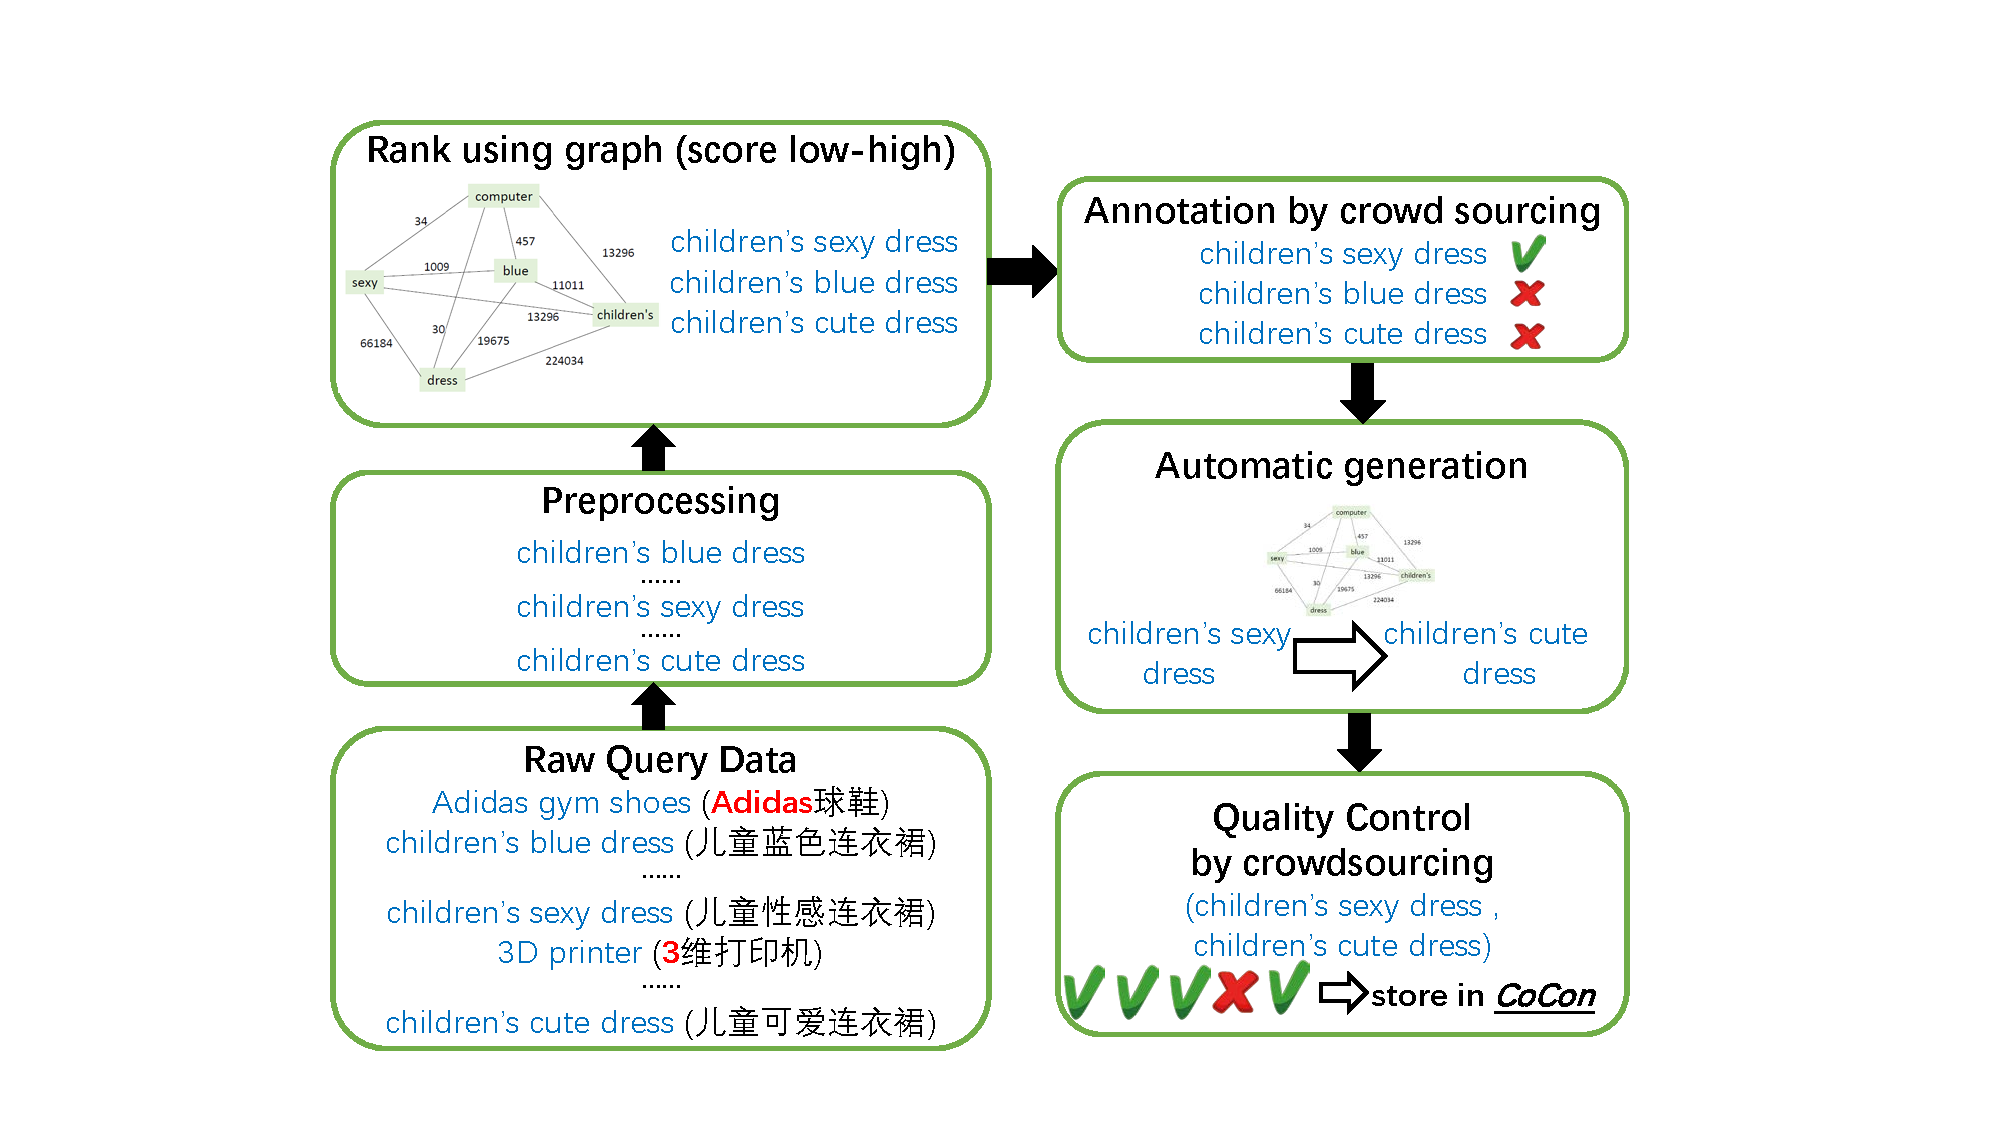
\includegraphics[width=\columnwidth]{images/framework.pdf}
	\caption{CoCo dataset collection process}
	\label{fig:framework}
\end{figure}

\subsection{Dataset Introduction}
Each instance in our CoCo dataset is %composed of 
%two short phrases and one label
a triple: $\{p_1, p_2, l\}$,
%Formally, each instance in our CoCo dataset is composed of 2 short phrases and 4 options: $\{p_1, p_2, r_1, r_2, r_3, r_4\}$. 
where $p_1$ and $p_2$ are two similar phrases focusing on the same subject
but with different modifiers.
However, only one of them is more plausible according to common sense. 
$l$ is the label which indicates the index of correct phrase. 
Therefore, the whole task can be seen as a binary classification problem 
and we use Accuracy as evaluation metric. 
%For the more unreasonable one, four options $\{r_1, r_2, r_3, r_4\}$ are offered to be chosen as the reason of being unreasonable. For both tasks, we use accuracy score to do the evaluation.
%\mx{Absence of dataset size}

\subsection{Raw Data Preprocessing}
%Alibaba inc offers us 
%We crawl %\mx{How to say??} 
We crawl search queries from a popular e-commerce platform 
where some noisy and meaningless queries are filtered
through query normalization including lexical error corrections and query rewriting.
We further filter out qeuries including numbers and English chars and remain  those queries that only composed of Chinese characters. 
After that, 4,081,254 common queries are left. 
These queries contain characters of length in range of 2 to 15, and 4.73 on average. The number of words\footnote{Word segmentations are done by using tools trained on E-commerce data in advance.} in queries is distributed between 2 to 8 and 2.07 on average.
%As for the number of words, queries distribute between 2 to 8, and 2.07 on average, 
The details of char and word number distribution is shown in Figure \ref{fig:wordDist}. 

\JQ{图得改:标题samples要留吗 0??保留几位小数?}
%\mx{figure or table is needed for words 2-8 or chars?}

\begin{figure}
	\centering
	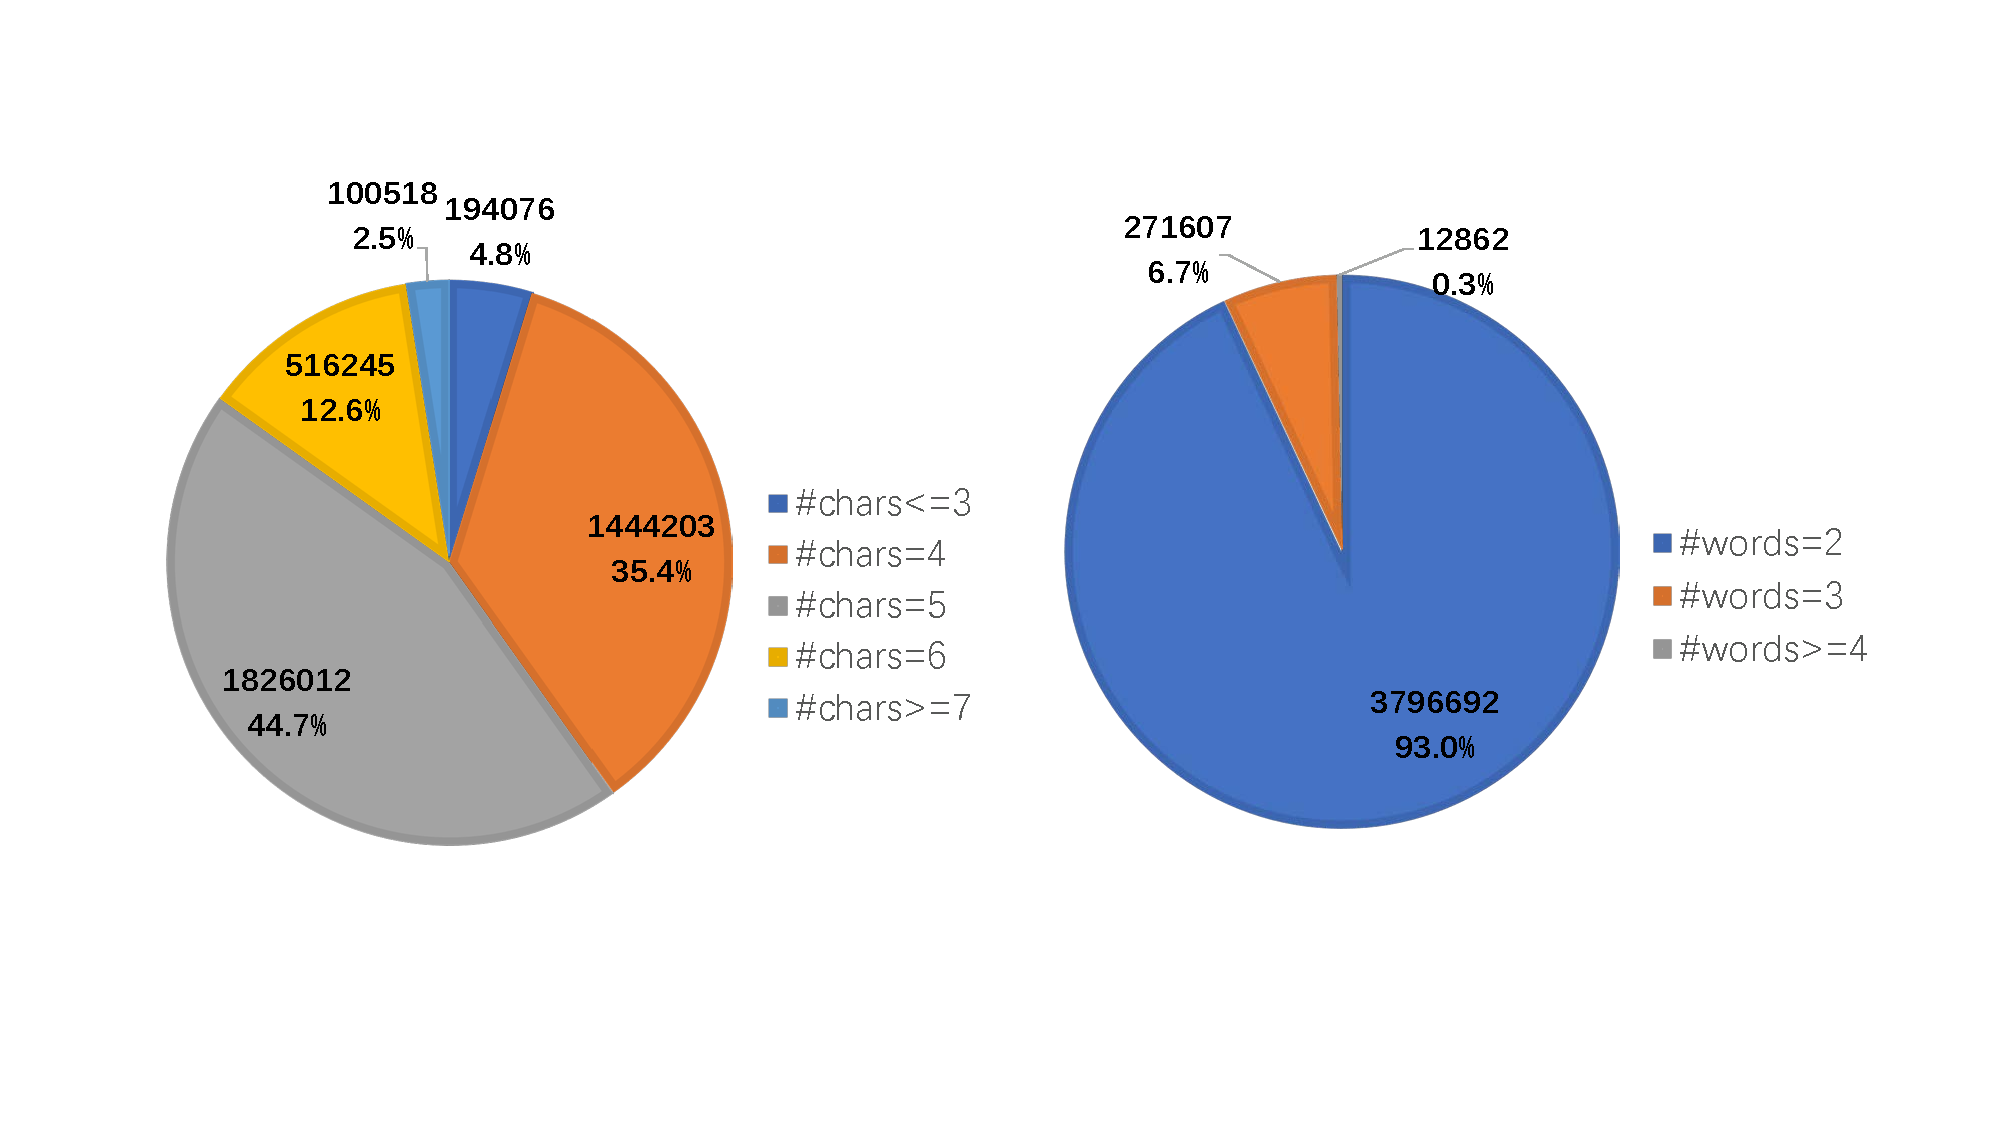
\includegraphics[width=0.95\columnwidth]{images/distributionWords.pdf}
	\caption{Char and word number distribution of raw data after preprocessing}
	\label{fig:wordDist}
\end{figure}

%\KZ{Words are too small in figure 1.}

%!!! Should give some statistics of this big table, ex. show length. 
%Besides, some modifications like query rewriting to make it clearer or lexical error corrections are also done. (query normalization) 


%\subsection{Preprocessed Data Overview}
\subsection{Auto-generation of CoCo pairs}
We define \textit{positive samples} as those phrases that have commonsense contradiction, and \textit{negative samples} as other phrases. 
%Our target is to get pairs of high-quality similar positive/negative samples as much as possible.
%Our target is to get positive samples as much as possible. 
%from the large query table.

To have a preliminary understanding over this whole table, we first randomly select 10,000 samples from preprocessed raw data and do the human annotation. 
%\mx{10000 need to be re-sampled, some samples that 1 word or have not-Chinese chars should be replaced.}
Among all selected samples, we find 292 positive samples and 9708 negative samples. It should be noticed that positive samples are much rarer than negative ones, only accounts for 2.92\%. Obviously, directly annotating the original collection of queries to get more negative\JQ{positive?} samples are not efficient.
%Therefore, we come up with two methods to get positive samples.
Therefore, we come up with two methods to get expected phrase pairs in CoCo dataset more efficiently: \textbf{Random generation} and \textbf{Filter using graph}. 

\subsubsection{Random Generation}
%As there are lots of negative samples, we consider to directly generate positive samples by randomly replacing 
%According to the statistics of preliminary human annotation, it is easier to get negative\JQ{positive} samples. %Hence, we consider 
The most nature and naive way is to directly generate associated similar positive samples starting with those negative annotated ones. %The following are our generation steps:
To check the effectiveness of this simple idea, we do the following experiments on a small dataset:
\begin{enumerate}
	\item Randomly select 100 high-quality negative samples, where \textit{high-quality} means:
	\begin{itemize}
		%\item [-] the query contains and only contains one subject, with one or several modifiers. For example, "skirt dress" is not satisfies because of two subjects; "cute dress" is a high-quality one.
		\item [-] \textit{stylistic} modifiers are clearly defined if exist, such as ``creative", ``personalized", ``popular" and etc.\JQ{有个stylistic modifiers字典之类的?}
		\item [-] modifiers in categories of \textit{nation} and \textit{color} should be paid more attention on. These two kinds of modifiers are versatile in most cases, for example, dress could be modified by all nations or colors, such as ``American dress", ``French dress", ``green dress" or ``red dress" and etc. However, some cases are special as they have intrinsic geographic characteristics (ex: ``Chinese dumplings") or color characteristics (ex: ``blue sea").\JQ{这个不是high-quality的标准吧?}
		\item [-] without brand name or people name. %(include actors).   
		\item [-] phrase is clear and the words used are common enough.	\JQ{common如何定义}
	\end{itemize}
	%\item To ensure that the candidate 100 negative samples are common and clear enough, we use official released "BERT-Base, Chinese" model \footnote{https://github.com/google-research/bert} to calculate perplexity of the choose 100 negative samples and replace those $PPL>=1000$ (9 among 100 for the first time) by other re-selected high-quality negative samples until all the selected negative samples satisfy $PPL<1000$. Here are the steps of calculating perplexity:
	%\begin{itemize}
	%	\item [-] As the vocabulary of original BERT Chinese model is on the level of characters, we just mask each character one by one for each query.
	%	\item [-] Fetch the probability of "MASK" being the associated character on the last layer, note as:\\$P(w_i) = P(w_i|w_1,...,w_{i-1},w_{i+1},...,w_n)$
	%	\item [-] For each query, we calculate perplexity as: \\
	%	$PPL(query) = e^{-(\sum_{i=1}^{n}logP_{i})/n}$  
	%\end{itemize}
	\item For each query, we randomly replace one of its word using vocabulary according to the following rules:
	\begin{itemize}
		\item [-] 
		%ensure consistency of word property itself, respecting the original Part-Of-Speech pattern. 
		ensure the consistency of the Part-Of-Speech pattern
		%which means subject replaced by subject, modifier replaced by modifier.
		\item [-] %ensure identity of word length, which means the replaced word should have the same length with the original word.
		ensure the identity of word length, because our further evaluation uses the perplexity (PPL) which is averaged by length during calculation. 
		%Notice that perplexity (PPL) is averaged by length during calculation, if one short modifier is replaced by a much longer modifier, even the new modifier does not match the subject, the new generated sample may get a lower ppl score as the new modifier itself is smooth and long enough to pull down the ppl score. Here is an example: "blue sky" vs "super cute green sky".
	\end{itemize} 
\end{enumerate}

Finally, ten positive samples are generated for each chosen negative sample, leading to 1000 pairs. We use one of the pretrained language model BERT to distinguish the more reasonable phrase from each pair. Perplexity (PPL) score is used as the evaluation metric: the pair with lower PPL will be considered as the more reasonable one.

Here are the steps of calculating PPL for a query $\{w_1 w_2 ... w_n\}$ by using the pretrained model BERT:
\begin{itemize}
	\item [-] As the vocabulary of original BERT Chinese model is trained on the level of characters, we just mask each character one by one for each query.
	\item [-] Fetch the probability of "MASK" being the associated character on the last layer\JQ{有点没看懂}, note as:\\$P(w_i) = P(w_i|w_1,...,w_{i-1},w_{i+1},...,w_n)$
	\item [-] For each query, we calculate perplexity as: \\
	$PPL(query) = e^{-(\sum_{i=1}^{n}logP_{i})/n}$  
\end{itemize}

There are totally 906 pairs that BERT judges correctly. The accuracy achieves 90.6\%. We also find that some pairs themselves can not be distinguished as both phrases are reasonable, such as ``Qing Dynasty teapo''(清朝茶碗) vs ``archaistic teabowl''(仿古茶碗). \JQ{这个pair怎么不符合generation呢}%The result shows that BERT really learns some useful statistical knowledge during pretraining stage.

However, after viewing all generated samples, %the randomly generated samples 
%they are indeed not high-quality 
they are indeed far away being a good dataset used for evaluating common sense, as there are some obviously strange combination such as ``cute shoe" vs ``bushy shoe", ``salty tofu" vs ``salty gypsum". \JQ{这个pair怎么不符合generation呢}
%this result also demonstrates that the randomly generated

Therefore, we decide to use another way to get pairs where phrases are more similar, more plausible, and with higher quality.

%\subsubsection{Further filter}
\subsubsection{Filter Using Graph}
%As statistics of human annotation show that there are only 2.92\% positive phrases if randomly sample from preprocessed raw data, directly annotation to get a large corpus of positive phrases are laborious. We aim at increasing the estimated proportion of positive samples and then applying human annotation to save time.

This method is based on the idea that \textit{popular query will have a larger probability to be reasonable}. We propose to construct a net of correlation weighted with co-occurrences between terms by using a large user queries corpus.

\textit{Step1: Positive samples preselecting}

%With the help of Alibaba inc, we obtain 
We first crawled user queries on e-commerce platform with data masking among 7 days (2019.07.15-2019.07.21). After filtering those queries that only have one word and keeping queries which are only formed by Chinese characters, we obtained 303,285,752 candidates in all. Then we analyze each query to get co-occurrence of each word pair, and gradually enrich the correlation net. 
For example, from the query ``sexy blue dress", we will get three word pairs (sexy, dress), (blue, dress) and (sexy, blue). Notice that the edge in our net does not have directions and the order of words is neglected.
% in word pairs is of no importance.
Besides, word synonyms are combined together using a Chinese synonym dictionary provided by HIT-SCIR\footnote{https://ltp-cloud.com/download/}.
After constructing net, the weight of each edge in the graph represents the frequency %number of times 
that this word pair was observed in the whole crawled user query corpus. A fragment of our constructed net is shown in Figure \ref{fig:net}.

\begin{figure}
	\centering
	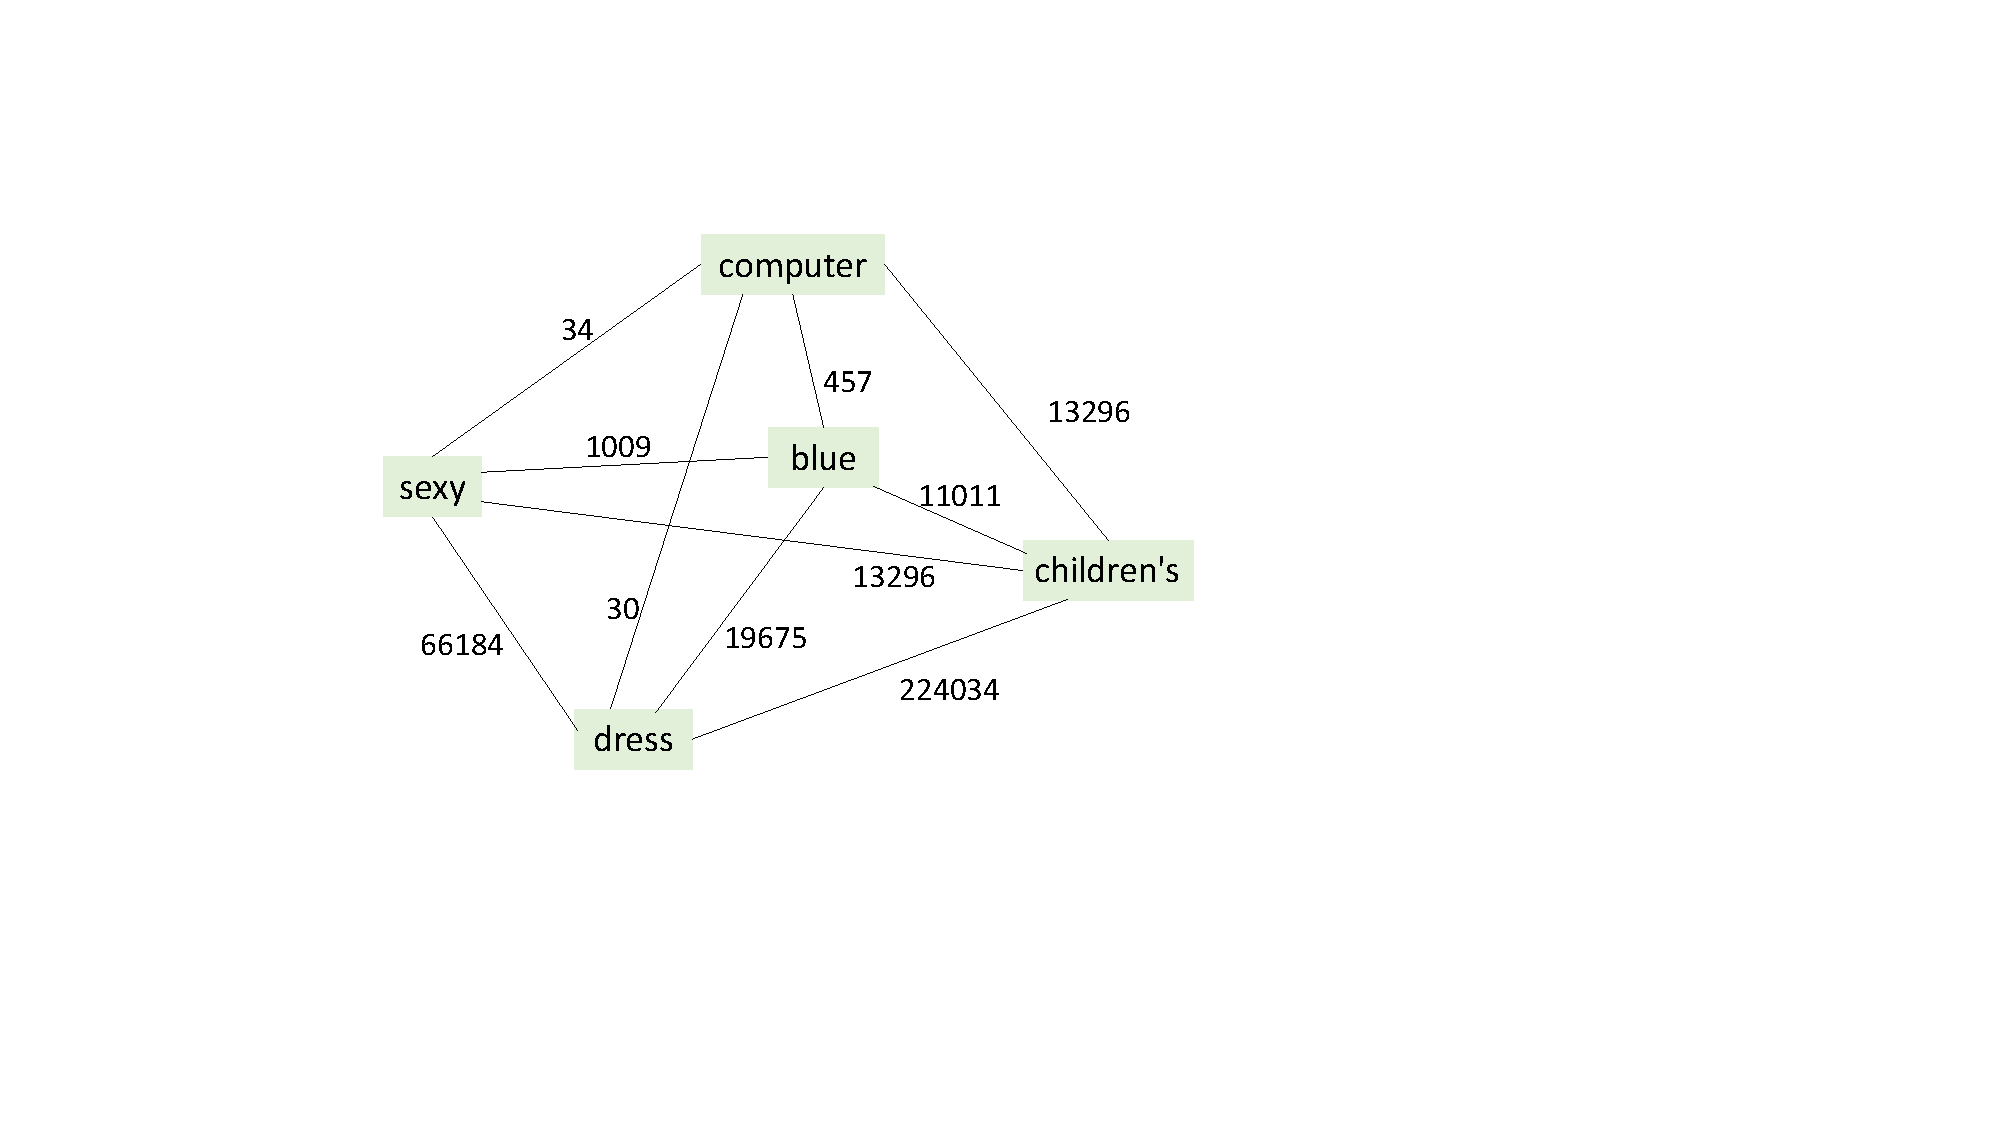
\includegraphics[width=0.8\columnwidth]{images/associationNetColor.pdf}
	\caption{A fragment of our constructed net}
	\label{fig:net}
\end{figure}

The distribution of users on the e-commerce platform is not uniform. For example, number of female users are much more than male users. This leads to the phenomenon that occurrence of word pair (electric, dress) may larger than (electric, torch) even though (electric, dress) is more unreasonable. The reason is that there are lots of female users search for \textit{dress} so even the strange combination of words may still appear much more times than a normal collocation with \textit{torch}. 
 
Mutual information is a suitable criterion to measure the dependency of two words. If word A appears $x$ times in the query corpus, word B appears $y$ times, the word pair (A,B) appears $z$ times, and the total number of words is $N$, then the mutual information between word A and B is defined as:
\begin{equation}
I(A,B) = log\frac{P_r(A\wedge B)}{P_r(A)\times P_r(B)}
\end{equation}
and can be estimated as:%using:
\begin{equation}
I(A,B) \approx log\frac{z\times N}{(x+z)\times (y+z)}
\end{equation}

We use mutual information to calculate the strength of word associations in our constructed net, which noted as ``plausibility".
%will be regarded as reasonability of this word pair.
%\KZ{Instead of reasonability, use the word ``plausibility''.}
For a phrase $T=(w_1, ..., w_m)$, there may not only two words, we need to calculate the overall plausibility $R$ as:
\begin{equation}
P(T) = \frac{2}{m*(m-1)}\sum_{i=1}^{m-1}\sum_{j=i+1}^{m}I(w_i, w_j)
\end{equation}

%Besides, as our positive sample should be clear, coherent and common, but a query may contain lots of noise,
%Besides, as there are countless combination of words, for example, the combination of \textit{color} and most daily things are reasonable, but the user query in 7 days may not cover all. Hence, we make another assumption after observing the result: Pair never appear $\neq$ unreasonable, BUT rare appear $=$ unreasonable. This assumption is a little strong but efficient for us to constrain the scope of positive samples.

%Hence we do not take the 2-word query into account \mx{should extend to 3 or more words phrase} if any word in the query or the word pair haven't appeared in our net.   

Besides, as most positive samples are common enough, we remove the phrase which contains any rare word that appears less than 100,000 in our graph. If all word pairs in a phrase doesn't exist in our graph, this phrase will also be filtered. Then, the remained samples are ranked according to their overall plausibility score from small to large to get the most unreasonable phrase list.

To evaluate the effectiveness of the above method, we test on our 10,000 preliminary annotated phrases. %as example.
After removing rare word, 6381 phrases (include 94 positive samples) are removed where the rate of positive phrase is 1.47\%. After removing non-exist word pair, another 107 samples (include 9 positive phrases) are removed. Finally, 3512 phrases (include 167 positive phrases) remain. Among previous 15\% of these samples, 77 positive ones among total 526 samples are found, where the rate of positive samples achieves 15.4\%, remarkably improves compared to 2.92\% on the 10,000 randomly selected on preprocessed raw data.
%showing the validity of the constructed graph.

%Therefore, we apply 
Seeing the validity of the constructed graph, the above method is applied on our whole unlabeled preprocessed 4,081,254 raw data, 1,176,922 are kept. After rank of overall plausibility score, %we fetch the previous 15\% (equals to 176,538 samples) for further human annotation.
we fetch the previous\JQ{front} 18,000 samples for further human annotation due to the limited resources.

%\subsection{Phrase annotation \& rewriting}
%When annotate and rewriting samples, annotator are both given a guideline to follow.

\textit{Step2: Phrase Annotation}

This part describes the guideline that the annotators are given to follow.
%During this period, annotators need to judge if a phrase is a commonsense contradiction. 
For given short phrases, annotators need to first filter the low-quality samples, then judge if it is an appropriate commonsense contradiction sample.\JQ{此句对吗}
\begin{enumerate}
	\item Phrase belongs to any one of these four cases can be directly ignored\JQ{deleted}: 
	%satisfies 
	\begin{itemize}
		\item [-] Reasonable phrase. %Correct commonsense phrase.
		\item [-] Not clear and can not distinguish the subject in a phrase, such as "children deer''(儿童麋鹿).\JQ{这条没懂}
		\item [-] Contain ambiguous subject, such as "cat" in "silk cat''(桑蚕丝猫咪), referring to an animal or an ornament.
		\item [-] Contain word that is too rare (i.e. unfamiliar to the annotator)
	\end{itemize}
	\item Judge the phrase to be unreasonable if it belongs to the four following commonsense contradiction category:
	\begin{itemize}
		\item [-] Several modifiers for one subject and commonsense contradiction exists between modifiers. For example, in ``Europe Korean curtain''(欧韩窗帘), two national modifiers are contradictory.
		\item [-] The modifier is contradictory with the intrinsic property of subject itself. For example, ``vitreous porcelain''(玻璃青花瓷), ``thermal ice bag''(保温冰袋), ``children sexy dress''(儿童性感连衣裙), ``boy night skirt''(男童睡裙).
		\item [-] The modifier is strange for describing the subject %'s intrinsic property 
		according to common sense, such as ``Walking alarm clock''(会走的闹钟), ``vacuum keyboard''(真空键盘).
	\end{itemize}
\end{enumerate}

%\KZ{You need to say how many human annotators are employed; what is the inter-judge
%agreement (assuming each entry is annotated by multiple judges.}
%Due to the resource limit, we only use the previous 18,000 of fetched data and distribute them to 6 person.  
We distribute these 18,000 fetched data to 6 person who is asked to choose intuitively the unreasonable phrase by their common sense. Finally, 15,567 commonsense contradiction samples are returned, hitting the rate of \textbf{86.48\%}, which is much larger than the original rate of \textbf{2.92\%}.

\textit{Step3: Negative Samples Generation}

Because human rewriting is costly, we consider a more efficient way to obtain the associated negative sample 
%(reasonable one) 
for each collected commonsense contradiction sample. The plausibility score $P$ is reused in this part: for each positive sample,
%(commonsense contradiction one)
we pair it with a short phrase in our total preprocessed query data that satisfies the following rules:
\begin{itemize}
	\item Describe the same object.
	\item Possess the same number of characters.
	\item Only one word in the original positive sample is replaced. %Only one word different from the original positive sample according to the result of segmentation.
	\item Plausibility score is higher than the original sample.
\end{itemize}

This automatic generation helps us to get 12,416 pairs of short phrases.

%\subsection{Additional Verification}
\subsection{Dataset Validation}
For further improving the quality of dataset, we ask different crowd workers to judge which phrase is more reasonable or can not distinguish between two phrases. We also set 300 checking problems. The annotated pairs from annotators who choose correctly on more than 80\% checking problems will be counted into the final collection. Figure \ref{fig:crowd} is the crowdsourcing web interface of data verification.\JQ{right?}

\begin{figure}
	\centering
	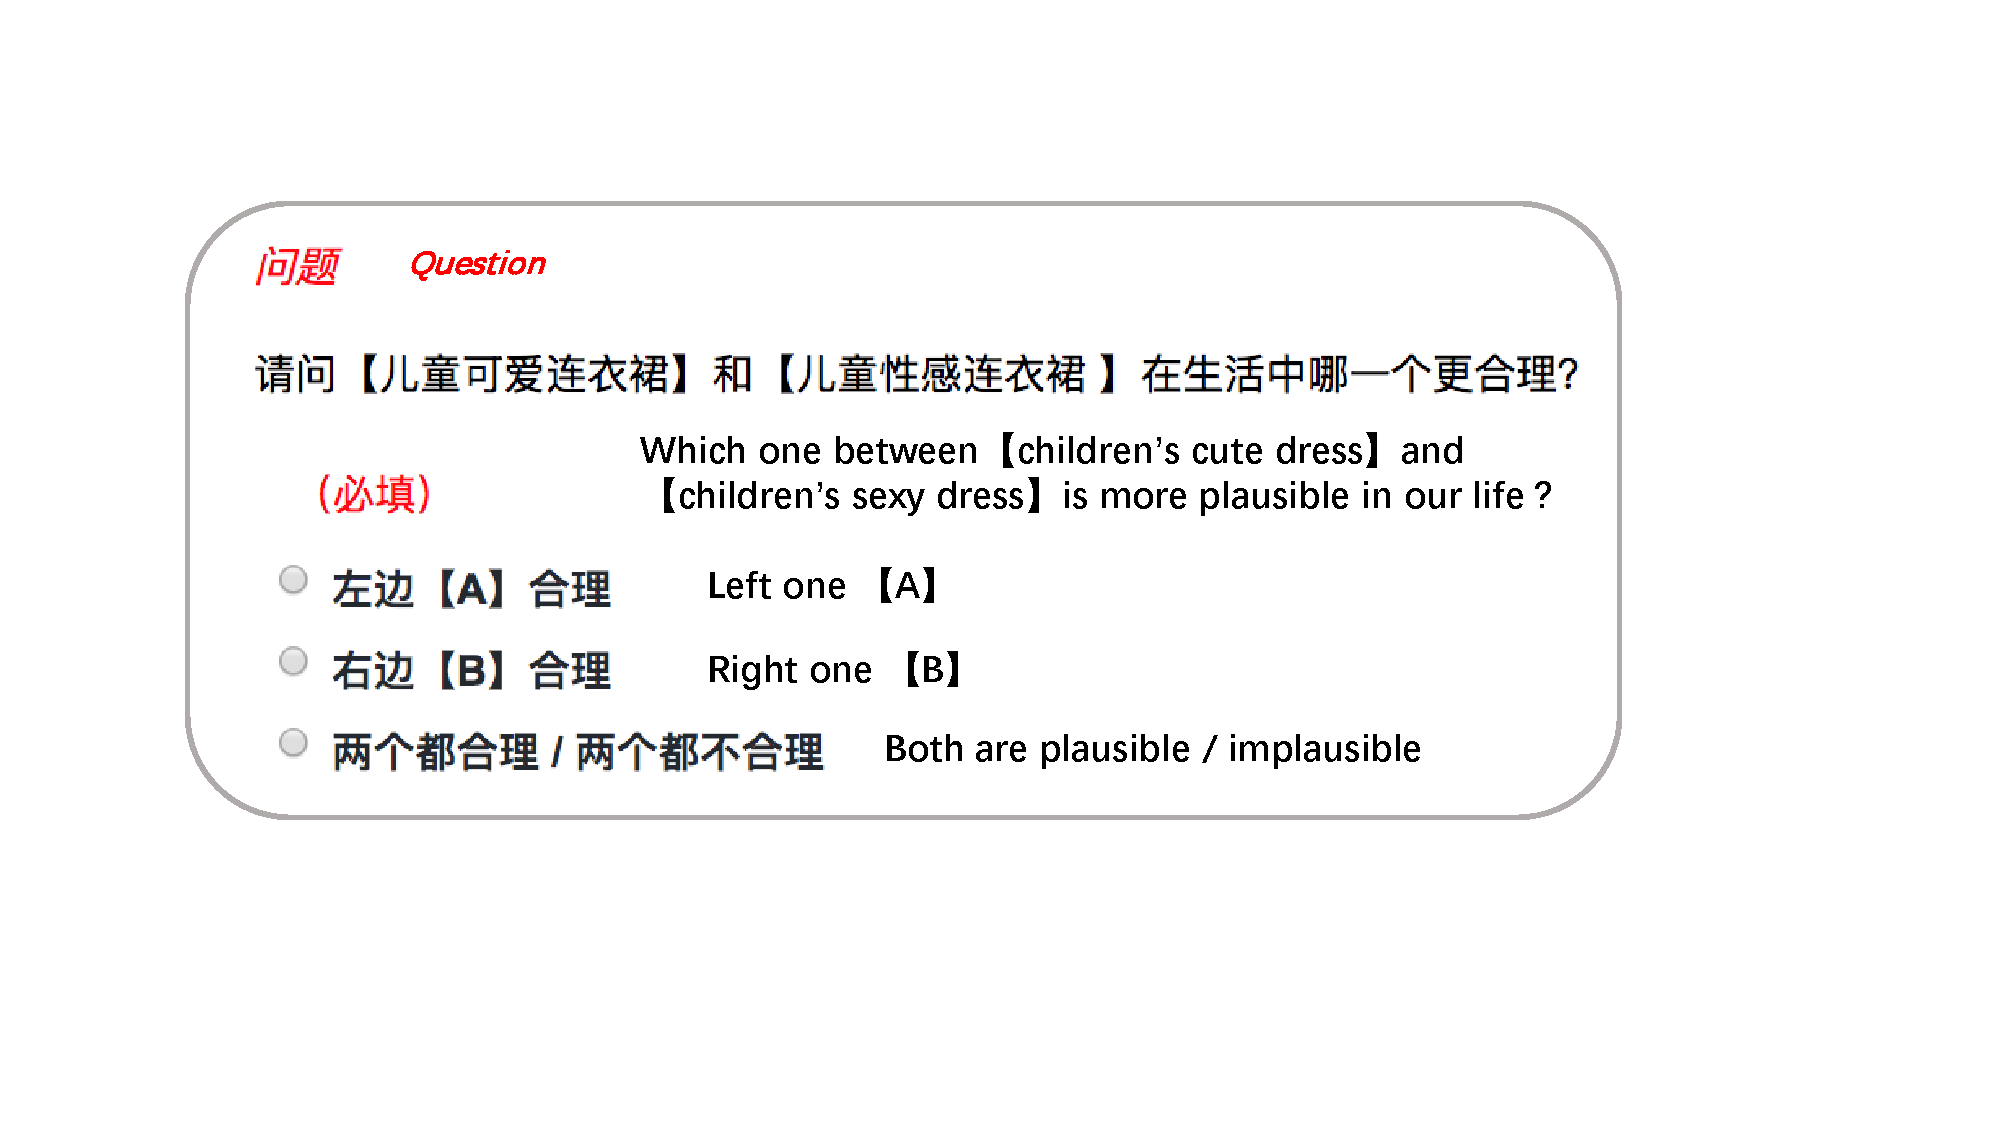
\includegraphics[width=0.95\columnwidth]{images/crowdPage.pdf}
	\caption{The crowd-facing web interface used to filter the dataset}
	\label{fig:crowd}
\end{figure}

Each sample is judged by 5 person, and we only keep those pairs that gain more than 4 same votes. After this step, we finally obtain our \textbf{CoCo} (\textbf{Co}mmonsense \textbf{Co}ntradiction) dataset, which contain 9,229 short phrase pairs \footnote{CoCo dataset can be found at \url{http://release_after_acception}}.


%\subsubsection{Phrase rewriting} After obtaining those commonsense contradiction samples, annotators are asked to rewrite them their relative negative ones which satisfy commonsense. For example, "sexy children dress" can be rewritten as "cute children dress". However, there are numerous rewrite ways. A rewrite is admitted if it accord with the following principles:
%\begin{enumerate}
%	\item Only one word is modified.
%	\item Do not modify the subject as subject is the core of phrase.
%	\item Property (include part of speech and type) of modified word should be the same with the original word. For example, verb should be changed to verb, same to noun, adjective and etc. The modified word should be similar with the original one in some aspect, which could confuse those pretrained model like BERT.
%	\item The replaced word should keep same length with the original word. Because we don't want length of word itself influence the judgement of model, either thick or dilute the weight of subject.
%	\item Try to avoid universal modifier in rewriting word, such as "personalized", "popular", color or nation. Because those universal modifiers hardly reveal any useful information for judgement. For example, human can not judge which is more reasonable between "personalized dress" and "popular dress" according to their commonsense knowledge.
%\end{enumerate} 

	\section{Analysis}
\label{sec:analysis}

% Analyze the main algo: time complexity, space complexity.
% Some properties to consider:
%
% \begin{itemize}
% \item give a bound on the total number of items suppressed;
% \item give a bound on the deviation in distribution from the original data;
% \item give a bound on the number of association rules that we eliminate;
% \item and what else??
% \end{itemize}

In this section, we show several interesting properties of our algorithm.
%in order to provide an all-aspect analysis of the problem and our algorithm.

%\begin{theorem}
%  The Optimal Suppression Problem in Definition \ref{def:osp} is NP-hard.
%\end{theorem}
%% TODO prove the whole problem hierarchy
%\begin{proof}
%  TODO
%\end{proof}

\begin{lemma}
\label{lemma:rule}
  If the inference $\mathcal{A}(q,a)$ is safe,
  then  $\mathcal{A}(q,a, b_1,b_2,\dots,b_n)$ is safe for any sequence of $\{b_i\}$.
\end{lemma}
\begin{proof}
  \begin{align*}
    \text{$q\rightarrow a$ is safe}
    \Rightarrow
    &\, \frac{\csize(q\cup\{a\})}{\csize(q)} \le \rho \\
    \Rightarrow
    &\, \csize(q\cup\{a\}) \le \rho\cdot\csize(q)
  \end{align*}
  \begin{align*}
    &\, (q\cup\{a\}) \subset (q\cup\{a, b_1,b_2,\dots,b_n\}) \\
    \Rightarrow
    &\,  \csize(q\cup\{a, b_1,b_2,\dots,b_n\}) \leq \csize(q\cup\{a\}) \le \rho\cdot\csize(q) \\
    \Rightarrow
    &\, \frac{\csize(q\cup\{a, b_1,b_2,\dots,b_n\}}{\csize(q)} \le \rho \\
    \Rightarrow
    &\, \text{$q\rightarrow a, b_1,b_2,\dots,b_n$ is safe}
  \end{align*}
\end{proof}

Lemma \ref{lemma:rule} shows that we do not have to consider rules with consequent of length 2 or longer.

\begin{lemma}%[Correctness of partitioning]
\label{CorrectnessOfPartitioning}
  If $q$ is safe in both $T_1$ and $T_2$, then $q$ is safe in $T = T_1 \cup T_2$.
\end{lemma}
\begin{proof}
For any item $a$,
  \begin{align*}
   q~\text{is safe in}~T_1 &\Rightarrow \csize_{T_1}(q\cup\{a\}) \le \rho\cdot\csize_{T_1}(q) \\
   q~\text{is safe in}~T_2 &\Rightarrow \csize_{T_2}(q\cup\{a\}) \le \rho\cdot\csize_{T_2}(q)
  \end{align*}
  So \begin{align*}
   \csize_{T_1}(q\cup\{a\}) + \csize_{T_2}(q\cup\{a\}) &\le \rho\cdot\csize_{T_1}(q) + \rho\cdot\csize_{T_2}(q)
  \end{align*}
  And \begin{align*}
    \csize_T(q\cup\{a\}) &= \csize_{T_1}(q\cup\{a\}) + \csize_{T_2}(q\cup\{a\}) \\
    \csize_T(q) &= \csize_{T_1}(q) + \csize_{T_2}(q)
  \end{align*}
  So $$ \frac{\csize_T(q\cup\{a\})}{\csize_T(q)} \le \rho~\Rightarrow q~\text{is safe in}~T .$$
\end{proof}

\begin{theorem}
\label{CorrectnessOfPartialSuppressor}
  \PartialSuppressor always terminates with a correct solution.
\end{theorem}
\begin{proof}
We first prove that if the algorithm terminates, the suppressed table is safe.
Note that the algorithm can only terminates on Line \ref{line:partial-suppressor-break}
  in Algorithm \ref{algo:partialsuppressor}.
So the value of $u$ on Line \ref{line:partial-suppressor-if-u} must always be \FALSE
  until the record cursor $i$ exceeds the table size $|T|$.
That means both \HandleShortRecords and \HandleLongRecord always return
  a pair with \FALSE as the first element during some pass of scanning of the whole table.
For \HandleShortRecords, returning \FALSE on Line \ref{line:handle-short-return-false}
  in Algorithm \ref{algo:handleshort} indicates there is no unsafe \qid in the buffer $B$.
For \HandleLongRecord, returning \FALSE on Line \ref{line:handle-long-return}
  in Algorithm \ref{algo:handlelong} indicates all the \qids generated by \Enum are safe.
So these return values of the two functions indicate there is no unsafe \qid in the table.
Hence, the suppressed table is safe.

Then we prove that \PartialSuppressor always terminates by measuring the
  number of items left (denoted $l$) in the table after each step of suppression.
Initially, $l=l_0=\sum_{i=1}^{|T|} |T[i]|\le |D| |T|$.
We state that for every invocation of \SanitizeBuffer, Line \ref{line:sanitize-suppress}
  in Algorithm \ref{algo:sanitize} is always executed at least once.
So the value $l$ strictly decreases when \SanitizeBuffer is invoked.
And before the table becomes safe, \SanitizeBuffer will be invoked for
  every iteration of the loop in Algorithm \ref{algo:partialsuppressor}.
So $l$ strictly decreases for each loop iteration in \PartialSuppressor.
Because $l$ starts from a finite number which is at most $l_0=\sum_{i=1}^{|T|} |T[i]|$,
  \PartialSuppressor must terminate.
Otherwise there will be an infinite descending chain of all the $l$ values.

Now we prove that Line \ref{line:sanitize-suppress} in Algorithm \ref{algo:sanitize}
  is always executed once \SanitizeBuffer is invoked.
Whenever \SanitizeBuffer is invoked, it is guaranteed that there exists
  an unsafe \qid $q\in B$ (see Line \ref{line:handle-short-if-contains-unsafe} in Algorithm \ref{algo:handleshort}
  and Line \ref{line:handle-long-if-contains-unsafe} in Algorithm \ref{algo:handlelong}).
$q$ is unsafe so that there always exists an item $e\in\linked(q)$ such that $P(e|q)>\rho$,
  i.e. \[ \frac{\csize(q\cup\{e\})}{\csize(q)}>\rho \Rightarrow \csize(q\cup\{e\})-\rho\cdot\csize(q)>0 .\]
For $k$ on Line \ref{line:sanitize-k1} in Algorithm \ref{algo:sanitize},
  \[ k = |X|-\lfloor\rho\cdot\csize(q)\rfloor = \csize(q\cup\{e\})-\lfloor\rho\cdot\csize(q)\rfloor \ge 1 .\]
For $k$ on Line \ref{line:sanitize-k2} in Algorithm \ref{algo:sanitize},
  it is guaranteed that the number of deletions is at least 1
  because the rule $q\rightarrow e$ is unsafe and there must be some deletions to make it safe.
So $k\ge 1$ on Line \ref{line:sanitize-while-k} for the first time.
Thus the condition is satisfied and Line \ref{line:sanitize-suppress} is executed.
\end{proof}

\begin{corollary}
The divide-and-conquer optimization \SplitData is correct.
\end{corollary}
\begin{proof}
It follows directly from Lemma \ref{CorrectnessOfPartitioning} and
Theorem \ref{CorrectnessOfPartialSuppressor}.
\end{proof}

%\begin{theorem}
%Let %$M = |T|$ be the size of table $T$,
%$l$ be the average record length,
%$c = r_r r_d$ where $r_r$ is the regression rate and $r_d$ is the qid duplicate rate.
%The average time complexity of \PartialSuppressor is
%\[ O(c \cdot 2^l |T|^2 l (\bmax (1-\rho) + l)). \]
%\end{theorem}
%\begin{proof}
%{\small\begin{verbatim}
%  general idea:
%  l1 <- estimate the number of iterations
%    for the loop in algorithm 1 -- assume
%    there is a parameter: regression ratio
%  may have to assume the data in some distribution
%    (e.g. power-law) -- related to Figure 1
%    count the number of invocations of HandleShort
%      --> b_max
%    count the number of invocations of HandleLong
%  l2 <- estimate the number of iterations
%    for the loop in algorithm 3
%  l1+l2 -> the number of invocation of SanitizeBuffer
%  estimate complexity of SanitizeBuffer
%  estimate complexity of line 7 to 13 in algorithm 3
%    (related to distribution in Figure 2)
%  estimate the complexity of UpdateBuffer
%\end{verbatim}}]

%Let $n_1$ be the number of short records,
%$n_2$ be the number of long records,
%$p(i)$ be the probability of a record being length $i$,
%$l_m$ be the maximum record length,
%$t=1-\rho$.
%
%Let $v_1$ be the number of invocations of \HandleShortRecords.
%In the process of generating qids and filling them into the qid buffer $B$,
%duplicates cannot be counted.
%If duplicates are allowed, the number of qids generated by a record is
%just $r=\sum_{i=1}^{\lmin-1} p(i)\cdot\#qid(i)$ where
%$\#qid(i)$ is the expected number of qids generated by a record of length $i$.
%Then $\bmax/r$ records are used to fill the buffer (duplicates allowed).
%So roughly $v_1=\frac{n_1\cdot r}{\bmax r_d}$ times to consider all distinct qids
%in short records, for a single pass.
%
%For \HandleLongRecord, the number of invocations is $v_2=n_2$ if
%we do not take multiple passes of table scanning (i.e., the loop in algorithm 1) into consideration.
%Assume the loop in \HandleLongRecord is iterated for $v_3$ times, then \SanitizeBuffer is
%roughly invoked for $v_1 + v_2 v_3$ times.
%
%There are 4 major parts in the computation. We will consider them one by one.
%
%The first part is Line 4 to 7 in Algorithm 2, since the buffer capacity is $\bmax$,
%the maximum number of iterations here is roughly $\bmax r_d$.
%\HandleShortRecords will be invoked for $v_1$ times, so
%the total time cost by this part of computation is roughly $v_1 \bmax r_d$.
%
%The second part is \UpdateBuffer in Algorithm 2. For the invocation
%$\UpdateBuffer(B, T, i, j, K, L)$, the purpose is to update $K$ and $L$
%by considering qids in records $T[i..j]$ which are also in $B$.
%So a single call invocation of \UpdateBuffer costs roughly $(j-i+1)|B|$.
%Hence, the total time cost by this part of computation is roughly
%$v_1 (|T| - \frac{\bmax}{r}) \bmax$.
%
%The third part is Line 7 to 13 in Algorithm 3. Note that in reality
%the computation from Line 10 to 12 can be done at the same time when
%calculating Line 8. And in the worst case, the total time cost by calculating
%these intersections is $\dnum l_m |T|$. And the total time cost by
%this part of computation is $v_2 v_3 \dnum l_m |T|$.

%The fourth part is all the invocations of \SanitizeBuffer.
%For a single invocation of \SanitizeBuffer, there are two sub-parts to consider.
%The first sub-part is the intersection calculation on Line 5 in Algorithm 4,
%which costs roughly $l |T|$.
%The second sub-part is the computation from Line 14 to 25 in Algorithm 4,
%which costs roughly $k |B|$, where $k$ is determined on Line $9$.
%In the worst case, $k= t |T|$.
%So for a single invocation of \SanitizeBuffer, the time cost is roughly
%$|B| r_r l (|T| L + t |T| |B|)$ where $|B|$ is the size of the buffer.
%Because \SanitizeBuffer is invoked $v_1$ times in \HandleShortRecords,
%with buffer size $\bmax$, and $v_2 v_3$ times in \HandleLongRecord,
%with buffer size $\dnum$,
%the total time cost by this part of computation is roughly
%$v_1 \bmax r_r l (l |T| + t |T| \bmax) + v_2 v_3 \dnum r_r l (l |T| + t |T| \dnum)$.
%
%Summing up these four parts we can get the following time cost.
%\begin{align*}
%  n_1 r
%+ \frac{n_1 (r |T| - \bmax)}{r_d}
%+ \frac{n_1 |T| r l r_r (\bmax t + l)}{r_d} \\
%+ l_m |T| n_2 \dnum v_3
%+ l |T| n_2 \dnum v_3 r_r (l + \dnum t)
%\end{align*}
%By eliminating non-denominating terms, we get the order of \[ O(c \cdot 2^l |T|^2 l (\bmax (1-\rho) + l) ) .\]
%\end{proof}
%
%For a given dataset, the expected time complexity is actually quadratic to the size of the table.

%\begin{theorem}
%  The space complexity of \PartialSuppressor on table $T$ is \[ O(\sum_{i=1}^{|T|} |T[i]| + \bmax) .\]
%\end{theorem}
%\begin{proof}
%Let $N = \sum_{i=1}^{|T|} |T[i]|$, then $N$ is the sum of the numbers
%of all item occurrences.
%This term is easy to explain since the algorithm has to store
%the original table $T$.
%So we only need to consider local data structures
%created in \PartialSuppressor
%and related functions for the term $O(\bmax)$.
%
%For \PartialSuppressor, the most significant memory cost is from the \qid buffer of size $\bmax$.
%For \HandleShortRecords, there is only $O(1)$ extra memory space for loop variables like $j$.
%For \HandleLongRecord, there is also $O(1)$ extra memory cost.
%For \SanitizeBuffer, except for the $O(1)$ memory space for local variables, it also involves
%  the storage of $\linked(\cdot)$ and $\csize(\cdot)$.
%Because all the \qids updated are from the buffer $B$, the total number of \qids being active at any time
%  is no greater than the capacity of the buffer, i.e. $\bmax$.
%In order to keep the information of $\linked(\cdot)$ and $\csize(\cdot)$,
%  there will be $O(\bmax)$ extra memory space used.
%\end{proof}

%\begin{theorem}
%  The algorithm suppresses at most $O(xxx)$ item occurrences on average.
%\end{theorem}
%\begin{proof}
%  TODO
%\end{proof}
%
%\KZ{Say something about the property of regression?}
%
%\KZ{A property for DnC time performance? The experiment seems to show that
%time decreases exponetially with $t_{max}$ for Retail, which is amazing!}

%\begin{property}
%  Idea: distribution similarity ...
%\end{property}
%\begin{proof}
%  TODO
%\end{proof}

	\section{Experiments}
\label{sec:exp}
We choose two state-of-the-art models BERT \cite{devlin2018bert} and ERNIE \cite{sun2019ernie} as our baselines. 

BERT is absolutely a milestone in NLP domain. Lots of NLP tasks achieve great improvements with BERT due to its pre-trained knowledge on natural language, including syntax and semantic features. 
Following the structure of pre-trained language model, some other works such as ERNIE and XLNet \cite{yang2019xlnet} come up to further improve the performance of BERT. 
Since training from scratch %on a large corpus 
is time-consuming, we choose the only two publicly released models pre-trained on Chinese corpus, \textbf{\textit{BERT-Base for Chinese}}\footnote{https://github.com/google-research/bert}  and \textbf{\textit{ERNIE 1.0 Base for Chinese}}\footnote{https://github.com/PaddlePaddle/ERNIE} as our baselines, 
%as they are the only two publicly released models pre-trained on the Chinese corpus,
where BERT is trained on Chinese wikipedia and ERNIE is trained on Chinese Wikepedia, Baidu Baike, Baidu news and Baidu Tieba. 
% trained dataset these two models use
%On the basis of BERT, ERNIE further modeled entity and word information to integrate knowledge to some extent.
As these two models are pre-trained using large corpus, we %first 
suppose that they have implicitly learned common sense.%\JQ{commonsense, finetune分分合合}

For our task, we calculate perplexity of phrase $\{w_1, w_2, ..., w_m\}$ %using the pre-trained language model 
by applying the following formula:
\begin{equation}
\label{ppl}
\begin{split}
&perplexity(phrase) = p(w_1, w_2, ..., w_m)^{-1/m} \\
&\approx \sqrt[m]{\prod_{i=1}^{m}\frac{1}{p(w_i|w_1,...,w_{i-1},w_{i+1},..., w_m)}}
\end{split}
\end{equation}
and we choose the one with higher score as the commonsense contradiction phrase.



\subsection{Fine-tune using E-commerce data}
Our dataset are collected from user query on an E-commerce platform. Although the data cover numerous scenarios in daily life, the word distribution is different from Chinese Wikipedia that used in the pre-training process of BERT and ERNIE. Therefore, we use the E-commerce data to fine-tune the model. The details of data used are shown in the Table \ref{tab:DetailData}.

As the training process are very slow due to the large data size, we only conduct the fine-tune process on BERT.% model.

\begin{table}
	\small
	\centering
	\begin{tabular}{cc}
		\toprule[1.1pt]
		Data source & Data Size \\
		\hline
		XiaoHongShu\tablefootnote{XiaoHongShu: https://www.xiaohongshu.com/} & 15 millions \\
		Baidu Baike & 10 millions \\
		Tao GongLue\tablefootnote{Tao GongLue and E-commerce descriptions are both from Taobao: https://www.taobao.com/} & 6+ millions \\
		E-commerce descriptions & 3+ millions \\
		\bottomrule[1.1pt]
	\end{tabular}
	\caption{Details of E-commerce data used for fine tune}
	\label{tab:DetailData}
\end{table}
%\footnotetext[7]{XiaoHongShu: https://www.xiaohongshu.com/}
%\footnotetext[8]{Tao GongLue and E-commerce descriptions are both from Taobao: https://www.taobao.com/}

\subsection{Fine-tune using CoCon dataset}
As we know that, human acquire common sense from his experience or inference based on his knowledge, instead of being told that something is absolutely right. Our released benchmark is also designed to measure if a machine has the commonsense judgment. Hence, we argue that common sense of machine should be learned implicitly from large corpus or inferred by knowledge acquired from external knowledge base, instead of tuning on a specific similar training set.
%in ConceptNet or Probase. 
%It should be noticed that the commonsense concerned more about the intrinsic property of things instead of some facts.  

However, we are also curious about how much the pre-trained language model like BERT can learn from short text. Therefore, we split our dataset into train/dev/test set and use train set to fine-tune the basic BERT and ERNIE.

To avoid the statistical clues revealed by word, we count frequency of each word that appears in either positive or negative side for each sample. Those words, which appear 1.5 times on one class more than another class, will not be put into the train set and test set simultaneously.
%Those words that have obvious statistical feature will not appear in the train set and test set simultaneously.
Finally, the data size of our train/dev/test set are 8343/454/432. %The results of fine-tuned BERT/ERNIE using all CoCon training data are shown in Table \ref{tab:ExpRes}. Besides, the learning curves with varying amounts of  training data will be presented and discussed in the last part of this section.  

For both BERT and ERNIE, we fine tune the network by adding a fully-connected layer over the first token obtained by the last layer in the original model, which is shown in Figure~\ref{fig:tuneNet}, where $S$ is the score obtained by fully-connected layer after softmax function. Because our task needs to compare two phrases in a data sample, hinge loss $L$ is used to do the optimization with threshold $\gamma$ equals to $0.5$. Initial learning rate of both models are set to be %$2e-5$
$2\mathrm{e}{-5}$, and the training epoch is 3. Other parameters are the same as the default settings given by the official tutorial.

\begin{figure}[h!]
	\centering
	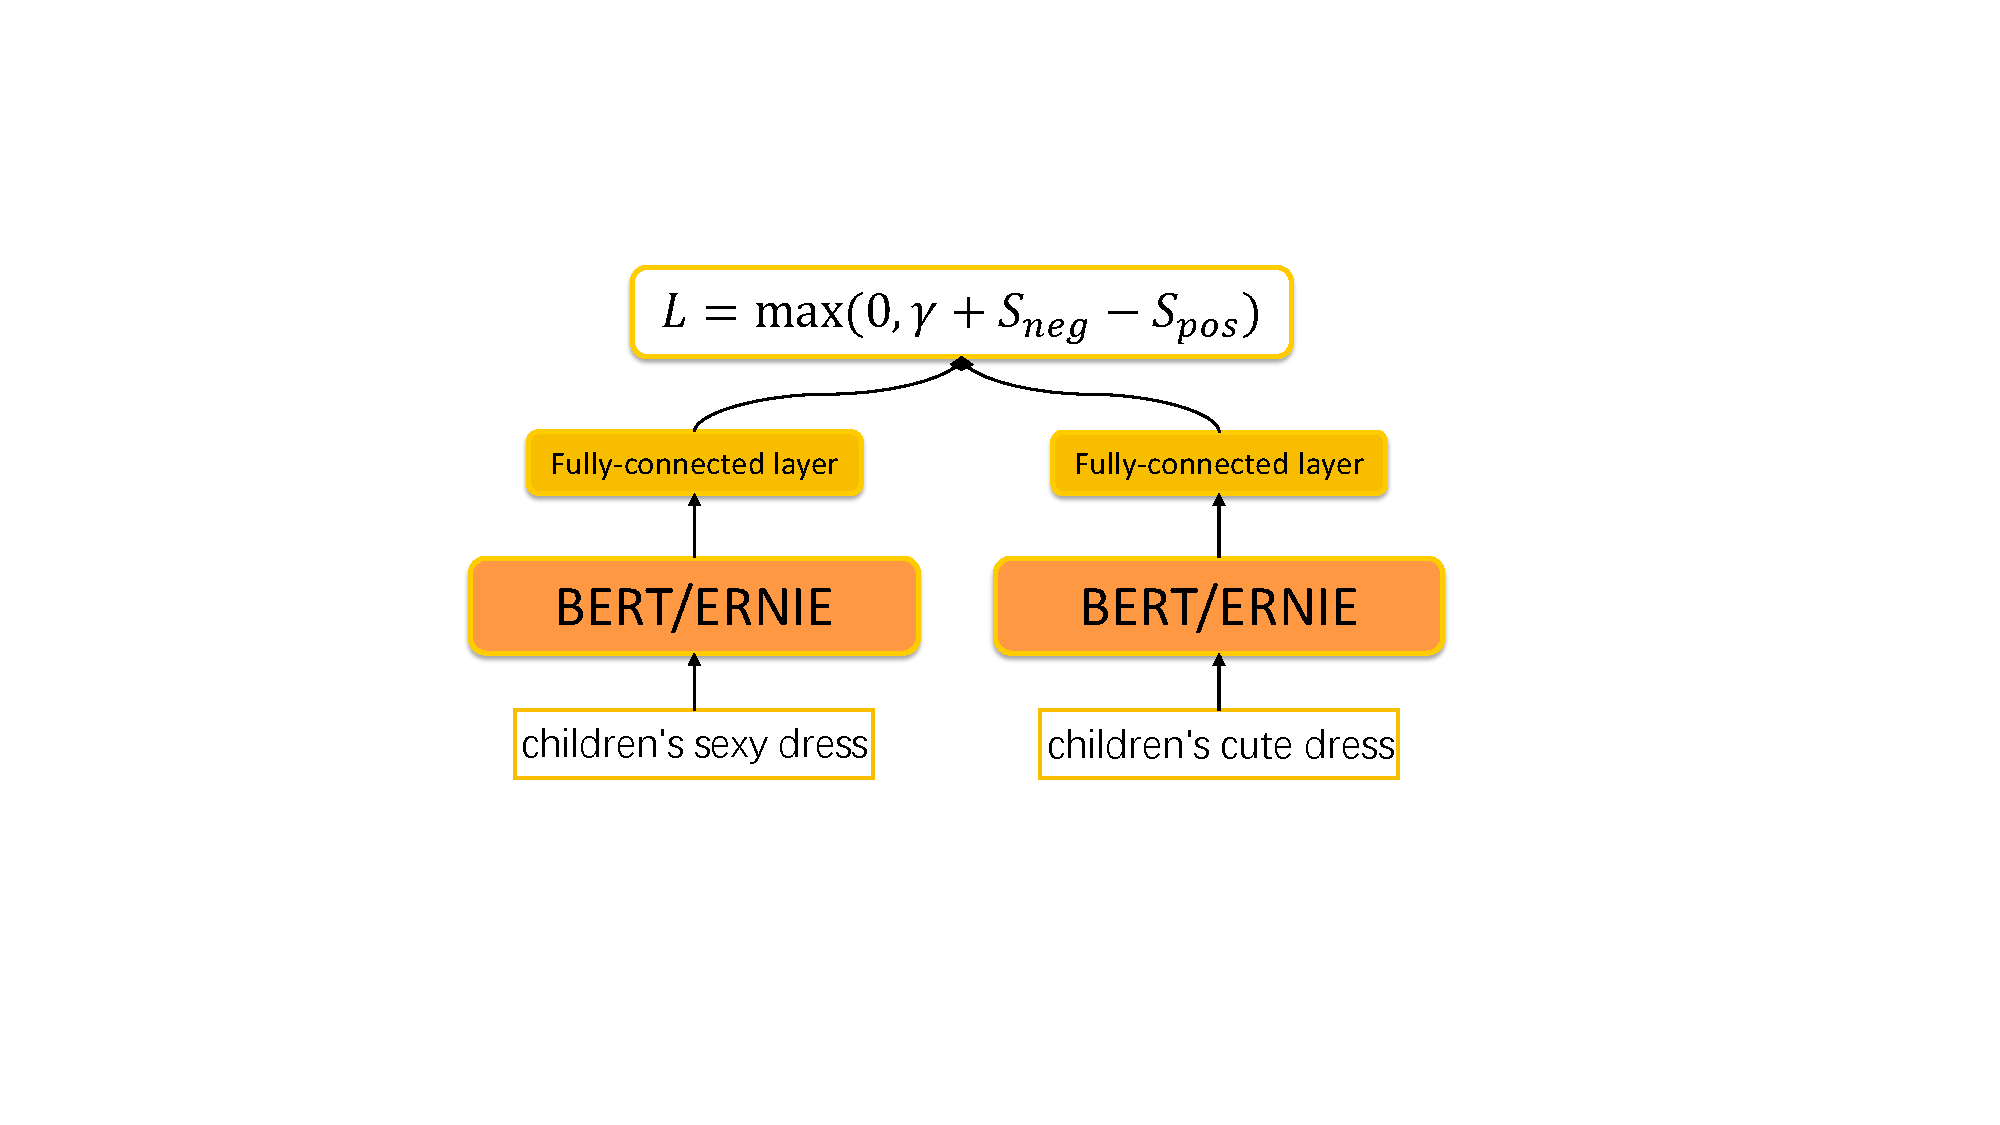
\includegraphics[width=0.8\columnwidth]{images/fineTuneNetwork.pdf}
	\caption{Model of Fine-tuned BERT\&ERNIE}
	\label{fig:tuneNet}
\end{figure}
%\KZ{translate the chinese in the figure to English.}
%\subsection{Experimental Setup}


\subsection{Human Evaluation}
We also conduct human evaluation on our dataset. 100 samples are randomly selected from dataset and distributed to two people, who did not participate in the construction or quality verification process of the dataset. The average of their accuracy are considered as the human performance borderline. 
%Results of experiments are shown in Table \ref{tab:ExpRes}.


\subsection{Results \& Analysis}
Results of all models are shown in Table \ref{tab:ExpRes}. As this is a binary classification problem, the random selection can achieve 50\% accuracy rate. 
The best baseline evaluated on CoCon dataset achieves accuracy of 0.6447. When fine-tuned on CoCon train set is permitted, the best baseline can achieve accuracy of 0.7662 on CoCon test data. However, these two results are both far below the human performance (0.95), demonstrating that our released benchmark is much easier for human, but still remains a great challenge for current state-of-the-art machine. Notice that all results surpass the random choice (0.5), showing that the pre-trained model %can indeed 
try to memorize numerous amounts of information.

\begin{table}
	\small
	\centering
	\begin{tabular}{p{4.3cm}p{1.4cm}p{1.4cm}}
		\toprule[1.1pt]
		Models & Accuracy (CoCon) & Accuracy (CoCon testset) \\
		%Models & Accuracy on CoCon & Accuracy on CoCon testset\\
		\midrule[0.75pt]
		Random & 0.5 & 0.5\\
		%\hline
		BERT & 0.5992 & 0.6019\\
		ERNIE & 0.6007 & 0.6944\\
		Fine-tuned BERT (E-commerce)  & \textbf{0.6447} & 0.6667\\
		Fine-tuned BERT (CoCon) & - & 0.7471\\ %0.7719\\
		Fine-tuned ERNIE (CoCon) & - & \textbf{0.7662} \\ %0.7847\\
		\midrule[0.75pt]
		Human&0.95&0.95\\
		\bottomrule[1.1pt]
	\end{tabular}
	\caption{Accuracy of models on CoCon dataset}
	\label{tab:ExpRes}
\end{table}


Without seeing any related data in CoCon train set and evaluated on the whole CoCon dataset, the basis pre-trained language model BERT (0.5992) and ERNIE (0.6007) perform nearly the same. 
The gap between these two models is considered due to the different size of pre-training data. As BERT uses only Chinese Wikipedia data, and ERNIE uses %another 
additional three data sources (include Baidu Baike/news/Tieba).  Except for Chinese Wikipedia, ERNIE may have seen more relation statistics between words. We also find that the accuracy of BERT improves after fine-tuning using E-commerce data, indicating that the dataset with more similar domain knowledge could further improve models' performance.

Despite of this small improvement, the performance of fine-tuned BERT using E-commerce data is still far from human. We argue that current design of pre-trained language model like BERT or ERNIE can not exactly learn commonsense knowledge from large amounts of training data, it needs to integrate external knowledge in some ways to be further %evaluated 
improved on our released benchmark. Besides, context-poor text also makes the task more challenging for machine to identify the contradiction.
%Besides, our dataset aimed at short text which also makes it more difficult for machine to understand directly as it is absent of enough context and standard syntactic structure.

%the fine-tuned BERT by E-commerce data achieves 

Take the split CoCon data into training process, both BERT and ERNIE get further improvement. The influence of varying amounts of training examples is shown in Section \ref{subsec:lr-curve}. %sub-section.   


%\subsection{Baseline Analysis}

\subsection{Learning Curves}
\label{subsec:lr-curve}

%To better understand the learning performance of both BERT and ERNIE, we fine-tune these two models on different size of CoCon training data.

To extrapolate how current two models BERT and ERNIE perform with various amount of data, we fine tune these two models by varying size of training set. We keep the number of training epochs, initial learning rate and the other hyper-parameters unchanged all the time. To deal with learning stabilities, each data point is the average of 4 runs. The resulting learning curves are plotted in Figure~\ref{fig:learnCurve}. 

We observe that the pre-trained ERNIE performs much better than BERT when the training samples are few, but their performance are getting close with increasing training data. 
The possible reason is that ERNIE tries to mask the entity and the whole word during its language model pre-training process, which may help ERNIE to better learn the relation between words. However the BERT only regard each Chinese character as a mask unit during pre-training. 

%The possible reason is that ERNIE use more training data during pre-trained process, may memorize more relation statistics between words. %However, ERNIE still defeats BERT little  

After using nearly 90\% of total dataset, these two models can merely achieve around 0.75, which is still substantially lower than human performance. Along the tendency of learning curves, large amounts of training samples are needed to approach human, neglecting the training convergence.
% We hypothesize that they will plateau quickly. (no instance)

%However, we hypothesize that both models need very large associated training data to 

\begin{figure}[h!]
	\centering
	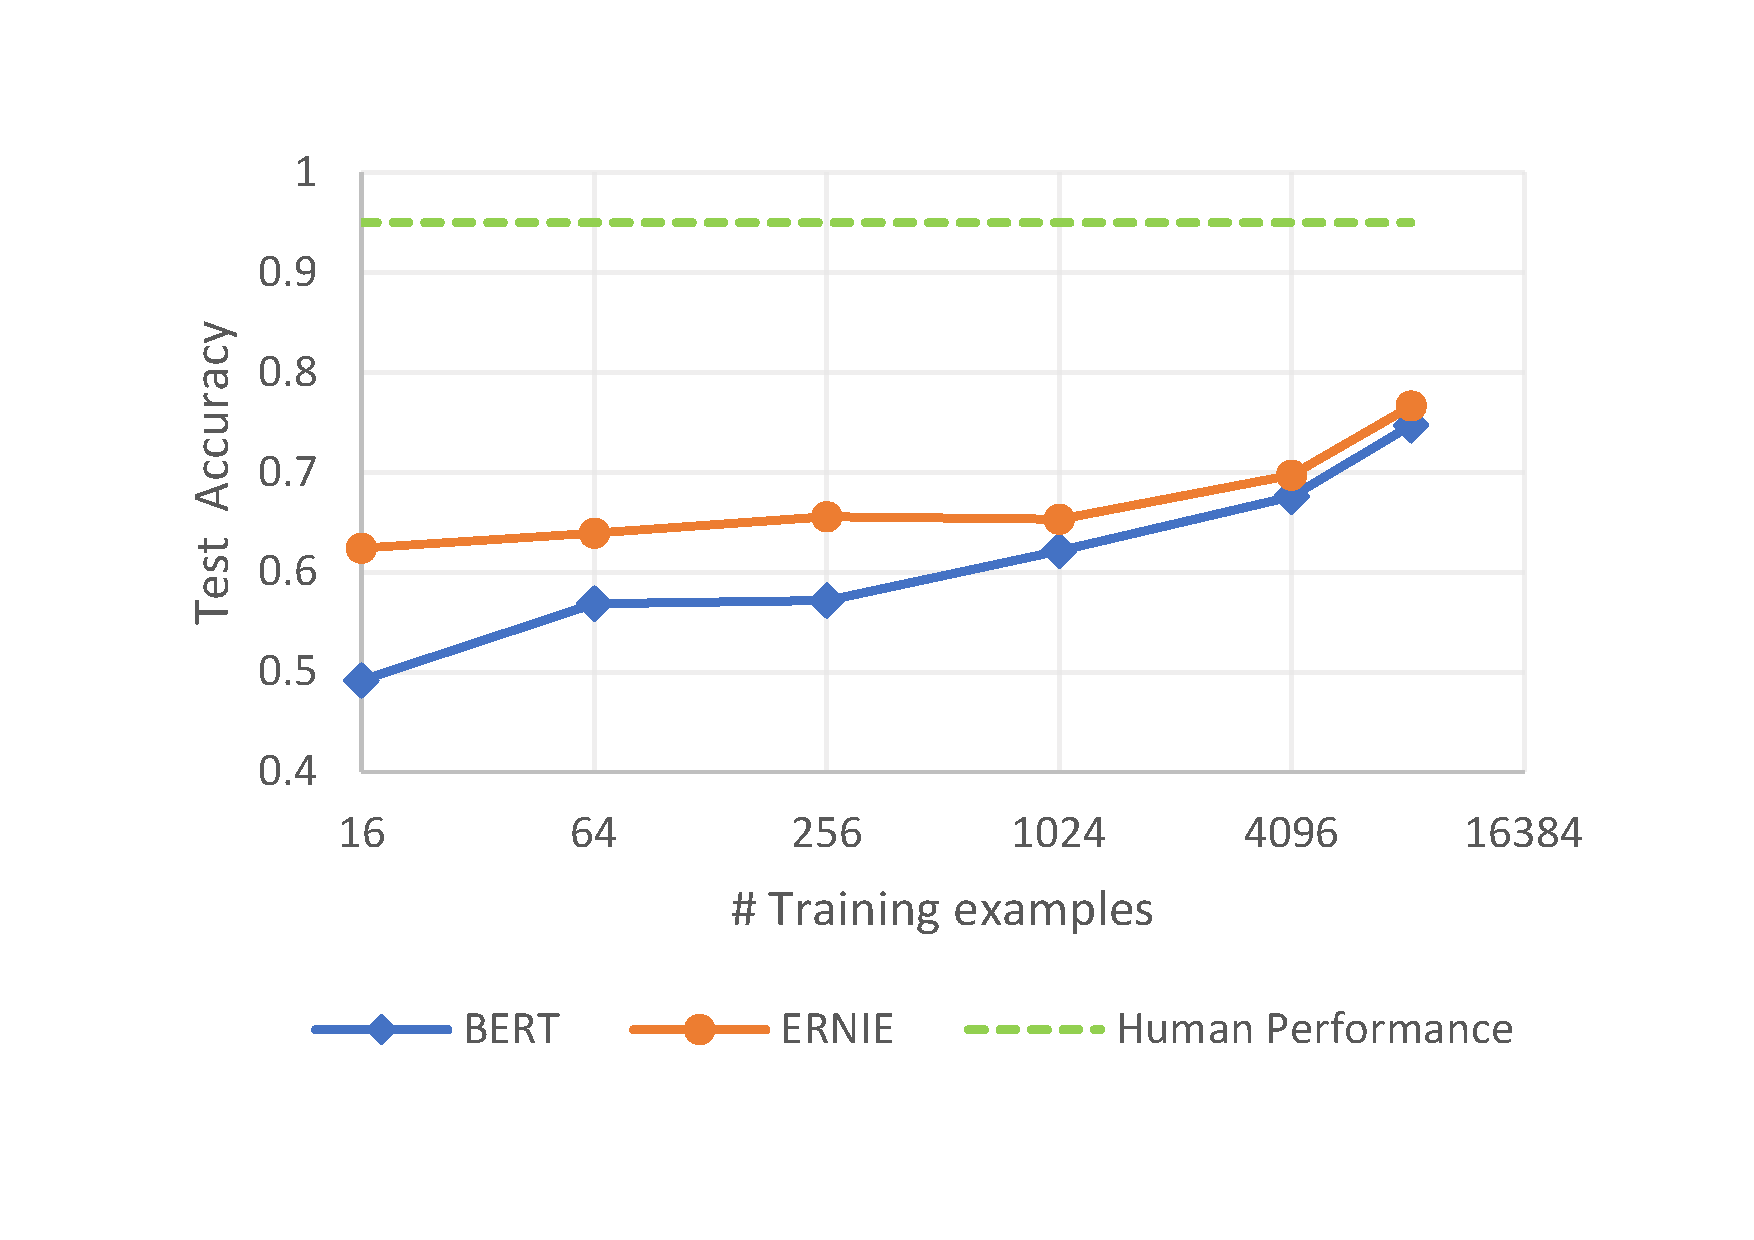
\includegraphics[width=0.85\columnwidth]{images/learnCurveLine.pdf}
	\caption{Accuracy on CoCon test set for BERT/ERNIE fine-tuned with varying amounts of data}
	\label{fig:learnCurve}
\end{figure}


	\section{Related Work}
\paragraph{Clarification Question Generation} The concept of CQ can be naturally raised in a dialogue system where the speech recognition results tend to be erroneous so that we raise CQs for sanity check \citep{stoyanchev2014towards}, or the intents for a task is incomplete or ambiguous in a first short utterance and further CQs are needed to fill in the slots \citep{dhole2020resolving}. The concept is then extended to IR to clarify ambiguous queries \citep{aliannejadi2019asking}, and has been successfully put into practice \citep{zamani2020generating}. Other application areas including KBQA \citep{xu2019asking} and open-domain dialogue systems \citep{aliannejadi2020convai3}. CQGen can also be applied to help refine posts on websites like StackExchange \citep{Kumar_2020} and Amazon \citep{rao2019answer}. In this context, our work closely follows the research line of \citep{rao2018learning, rao2019answer, cao2019controlling}. \citet{rao2018learning} first adopted a retrieval-then-rank approach. They \citep{rao2019answer} then proposed a generation approach to train the model to maximize the utility of the hypothetical answer for the questions with GAN, to better promote specificity. \citet{cao2019controlling} propose to control the specificity by training on data with explicit indicator of specificity, but it requires additional specificity annotation. Towards the similar specificity goal, we adopted a different keyword-based approach. They also assume generating one question per context, which we claim is not sufficient to cover various possible information needs, and thus propose the task of the diverse CQGen.

\paragraph{Diverse Generation} The demand for diverse generation exists in many other fields~\cite{vijayakumar2018diverse, LiangZ18code, shen2019mixture}, and we've drawn inspirations from these literatures. For image captioning, we may use multiple descriptions for different focusing points of a scene. \textit{Diverse Beam Search} \citep{vijayakumar2018diverse} was proposed to broaden the searching space to catch such diversity by dividing groups in decoding and imposing repetition penalty between them. For machine translation, a context can be translated with different styles. \citet{shen2019mixture} thus proposed \textit{Mixture of Expert} models including hMup to reflect various styles with a discrete latent variable (\textit{expert}). And here for CQGen, diversity is required to cover various potentially missing aspects, so we come up with the idea to use keywords as a controlling variable like \textit{expert} to promote diversity.


	\section{Conclusion}

In this paper, we incorporated the idea of Cookie Theft picture description task into the evaluation of the high-level cognitive abilities of LVLMs and designed a novel evaluation benchmark called CogBench.
% Images in CogBench are of high quality and require more cognitive reasonings to understand, which makes it different from existing image datasets.
The images in CogBench are of high quality and demand more complex cognitive reasoning for interpretation, setting it apart from existing image datasets.
% It consists of a image description task and a VQA task.
Experiments show that there is still a large gap between the cognitive abilities of LVLMs and human beings, indicating CogBench is a challenging benchmark.

% In the future

	
	\bibliographystyle{named}
	\bibliography{ijcai20}
	\end{CJK}

\end{document}
